% #############################################################################
% This is the MAIN DOCUMENT of the Thesis MSc TEMPLATE.
% The content for the Thesis MSc is to be written in separate documents
% located in the folder ./Chapters
%         Aknowledgments.tex
%         Abstract.tex
%         KeyWords.tex
%         Resumo.tex
%         PalavrasChave.tex
%         Acronyms.tex
%         Front_Cover.tex
%         Chapter_1.tex ....Chapter_2 .....
%         ApendixA.tex ... ApendixB.tex...
% -----------------------------------------------------------------------------
% The class "istulthesis" is based on the standard LaTeX 'report' class.
% It can be used for Instituto Superior Tecnico thesis, as it follows the 
% regulations published by the Scientific Council of IST.
% The class defines the document style. 
% IST requires the thesis to be written in Arial or similar. 
% Two arguments in '\documentclass' allow you to define the thesis font: 
% 'Helvetica' and 'AvantGarde', which transforms 
% the default LaTeX font into Helvetica or AvantGarde, respectively.
% #############################################################################
% The document is automatically set for english or portuguese by just selecting
% the MAIN LANGUAGE in file 'Thesis-MSc-Preamble_commands.tex' 
% #############################################################################
% Thesis-MSc
% Version 2.0, August 2018
% BY: Rui Santos Cruz, rui.s.cruz@tecnico.ulisboa.pt
% #############################################################################
% !TEX root = ./main.tex
% -----------------------------------------------------------------------------
%
\documentclass[defaultstyle,10pt,Helvetica]{istulthesis}
%
% -----------------------------------------------------------------------------
% The Preamble document contains all the necessary Packages for typesetting
% Modify it to suit your needs
% -----------------------------------------------------------------------------
% #############################################################################
% Preamble for Thesis-MSc in English or Portuguese
% Required Packages and commands
% --> Please Choose the MAIN LANGUAGE for the Thesis in package BABEL (below)
% !TEX root = ./main.tex
% #############################################################################
% Thesis-MSc
% Version 2.0, August 2018
% BY: Rui Santos Cruz, rui.s.cruz@tecnico.ulisboa.pt
% #############################################################################
%
% -----------------------------------------------------------------------------
% PACKAGES ucs, utf8x, babel, iflang:
% -----------------------------------------------------------------------------
% The 'ucs' package provides support for using UTF-8 in LaTeX documents. 
% However in most situations it is not required.
\usepackage{ucs}
% The 'utf8x' package contains support for using UTF-8 as input encoding. 
\usepackage[utf8x]{inputenc}
% The 'babel' package may correct some hyphenation issues of LaTeX. 
% Select your MAIN LANGUAGE for the Thesis with the 'main=' option.
\usepackage[main=english,portuguese]{babel}
% The 'iflang' package is used to help determine the language being used. 
\usepackage{iflang}

% -----------------------------------------------------------------------------
% PACKAGE scrbase:
% -----------------------------------------------------------------------------
% The 'scrbase' package is used to help redefining document structure.
\usepackage{scrbase}
% -----------------------------------------------------------------------------
% PACKAGE mathtools, amsmath, amsthm, amssymb, amsfonts, nicefrac:
% -----------------------------------------------------------------------------
% These packages are typically required. 
% Among many other things they add the possibility to put symbols in bold
% by using \boldsymbol (not \mathbf); defines additional fonts and symbols;
% adds the \eqref command for citing equations.
\usepackage{mathtools, amsmath, amsthm, amssymb, amsfonts}
\usepackage{nicefrac}
%
% -----------------------------------------------------------------------------
% PACKAGE tikz:
% -----------------------------------------------------------------------------
% Tikz  for creating graphics programmatically.
\usepackage{tikz}
\usetikzlibrary{shapes.geometric, arrows, positioning}
% -----------------------------------------------------------------------------
% PACKAGES array, booktabs, multirow, colortbl, ctable, spreadtab:
% -----------------------------------------------------------------------------
% These packages are most usefull for advanced tables. 
% 'multirow' allows to join rows throuhg the command \multirow which works
% similarly with the command \multicolumn.
% The 'colortbl' package allows to color the table (foreground and background)
% The 'ctable' package provides commands to easily typeset centered or left or
% right aligned tables.
% The package 'booktabs' provide some additional commands to enhance
% the quality of tables
% The 'longtable' package is only required when tables extend beyond the length
% of one page, which typically does not happen and should be avoided
\usepackage{array}
\usepackage{booktabs}
\usepackage{multirow}
\usepackage{colortbl}
\usepackage{ctable}
\usepackage{spreadtab}
\usepackage{longtable}
%
% -----------------------------------------------------------------------------
% PACKAGES graphicx, subfigure:
% -----------------------------------------------------------------------------
% The package 'graphicx' supports formats PNG and JPG.
% Package 'subfigure' allows to place figures within figures with own caption. 
% For each of the subfigures use the command \subfigure.
\usepackage{graphicx}
\usepackage[hang,small,bf,tight]{subfigure}
%
% -----------------------------------------------------------------------------
% PACKAGE caption:
% -----------------------------------------------------------------------------
% The 'caption' package offers customization of captions in floating 
% environments such figure and table
% \usepackage[hang,small,bf]{caption}
\usepackage[format=hang,labelfont=bf,font=small]{caption} 
% the following customization adds vertical space between caption and the table
\captionsetup[table]{skip=10pt}
%
% -----------------------------------------------------------------------------
% PACKAGE algorithmic, algorithm, algorithm2e:
% -----------------------------------------------------------------------------
% These packages are required if you need to describe an algorithm.
% The preference is for using 'algorithm2e'
%\usepackage{algorithmic}
%\usepackage[chapter]{algorithm}
\usepackage[ruled,vlined,algochapter,norelsize,\languagename]{algorithm2e}
%
% -----------------------------------------------------------------------------
% PACKAGE listings
% -----------------------------------------------------------------------------
% These packages are required if you need to list code snippets.
\usepackage{listings}
% Nicely syntax highlighted m-code in LaTeX documents with stylefile mcode.sty
% http://www.mathworks.com/matlabcentral/fileexchange/8015-m-code-latex-package
\usepackage[numbered]{./tables_and_code/mcode}
%
% -----------------------------------------------------------------------------
% Re-define listings captions and titles based on language.
\newcaptionname{portuguese}{\lstlistingname}{Listagem} % Listings CAPTIONS
\newcaptionname{portuguese}{\lstlistlistingname}{Listagens} % LIST of LISTINGS
%
% -----------------------------------------------------------------------------
% PACKAGE csquotes
% -----------------------------------------------------------------------------
% Quotation helper package
\usepackage{csquotes}
%
% -----------------------------------------------------------------------------
% PACKAGE todonotes
% -----------------------------------------------------------------------------
% Create TODO Notes in text
% The notes can be made invisible by just using the 'disable' option:
\usepackage[textwidth=2cm, textsize=small]{todonotes}
%\usepackage[textwidth=2cm, textsize=small, disable]{todonotes}
\setlength{\marginparwidth}{2cm}
%
% -----------------------------------------------------------------------------
% PACKAGE changes
% -----------------------------------------------------------------------------
% Track changes in document (changes in pdf preview).
%% Use "final" option to make all tracking markups invisible.
%\usepackage[authormarkup=superscript,authormarkuptext=id,markup=underlined,ulem={ULforem,normalbf},final]{changes}
\usepackage[authormarkup=superscript,authormarkuptext=id,markup=underlined,ulem={ULforem,normalbf}]{changes}
% commands:
% \added[id=xx]{text}
% \deleted[id=xx]{text}
% \replaced[id=xx]{deleted text}{added text}
% -----------------------------------------------------------------------------
% PACKAGES xcolor, color
% -----------------------------------------------------------------------------
% These packages are required for list code snippets.
\usepackage{xcolor}
\usepackage{color}
% The following special color definitions are used in the IST Thesis
\definecolor{forestgreen}{RGB}{34,139,34}
\definecolor{orangered}{RGB}{239,134,64}
\definecolor{lightred}{rgb}{1,0.4,0.5}
\definecolor{orange}{rgb}{1,0.45,0.13}	
\definecolor{darkblue}{rgb}{0.0,0.0,0.6}
\definecolor{lightblue}{rgb}{0.1,0.57,0.7}
\definecolor{gray}{rgb}{0.4,0.4,0.4}
\definecolor{lightgray}{rgb}{0.95, 0.95, 0.95}
\definecolor{darkgray}{rgb}{0.4, 0.4, 0.4}
\definecolor{editorGray}{rgb}{0.95, 0.95, 0.95}
\definecolor{editorOcher}{rgb}{1, 0.5, 0} % #FF7F00 -> rgb(239, 169, 0)
\definecolor{chaptergrey}{rgb}{0.6,0.6,0.6}
\definecolor{editorGreen}{rgb}{0, 0.5, 0} % #007C00 -> rgb(0, 124, 0)
\definecolor{olive}{rgb}{0.17,0.59,0.20}
\definecolor{brown}{rgb}{0.69,0.31,0.31}
\definecolor{purple}{rgb}{0.38,0.18,0.81}
%
% -----------------------------------------------------------------------------
% PACKAGE setspace:
% ----------------------------------------------------------------------------
% Provides support for setting the spacing between lines in a document. 
% Package options include single spacing, one half spacing, and double spacing. 
% Alternatively the spacing can be changed as required with:
% \singlespacing, \onehalfspacing, and \doublespacing commands
\usepackage{setspace}
%
% -----------------------------------------------------------------------------
% PACKAGE paralist
% -----------------------------------------------------------------------------
% This package provides the 'inparaenum' environment for inline lists
\usepackage{paralist}
% usage:
% \begin{inparaenum}[(a)]
% \item bla
% \item bla, bla
% \end{inparaenum}
% -----------------------------------------------------------------------------
% PACKAGE cite:
% -----------------------------------------------------------------------------
% The 'cite' package will result in citation numbers being automatically
% sorted and properly "ranged". i.e.,
% [1], [2], [5]--[7], [9]
\usepackage{cite}
%
% -----------------------------------------------------------------------------
% PACKAGE acronym:
% -----------------------------------------------------------------------------
% The package 'acronym' garantees that all acronyms definitions are 
% given at the first usage. 
% IMPORTANT: do not use acronyms in titles/captions; otherwise the definition 
% will appear on the table of contents.
\usepackage[printonlyused]{acronym}
%
% -----------------------------------------------------------------------------
% PACKAGE hyperref
% -----------------------------------------------------------------------------
% Set links for references and citations in document
\usepackage{hyperref}
% pre-configuration of hyperref
\hypersetup{ colorlinks=true,
             citecolor=cyan,
             linkcolor=darkgray,
             urlcolor=teal,
             breaklinks=true,
             bookmarksnumbered=true,
             bookmarksopen=true,
             pdftitle=\@title, % THESIS TITLE
             pdfauthor=\@author,  % YOUR NAME
             pdfcreator=\@author,   % YOUR NAME
}
%
% -----------------------------------------------------------------------------
% PACKAGE url:
% -----------------------------------------------------------------------------
% Provides better support for handling and breaking URLs.
\usepackage{url} 
%
% -----------------------------------------------------------------------------
% PACKAGE Cleveref:
% -----------------------------------------------------------------------------
% Clever Referencing of document parts
% Note: portuguese is supported through "brazilian" option
\usepackage[\IfLanguageName{english}{english}{brazilian}]{cleveref}
%
% -----------------------------------------------------------------------------
% PACKAGE enumitem:
% -----------------------------------------------------------------------------
%For enhanced enumeration of lists
%\usepackage{enumitem}
\usepackage[shortlabels]{enumitem}
\setlist[description]{leftmargin=\parindent,labelindent=\parindent,itemsep=1pt,parsep=0pt,topsep=0pt}
%
% #############################################################################
% GLOBAL FORMATTING OF THE THESIS DOCUMENT before using FANCY stuff
% Set paragraph counter to alphanumeric mode
\renewcommand{\theparagraph}{\Alph{paragraph}~--}
\hoffset 0in
\voffset 0in
\oddsidemargin 0 cm
\evensidemargin 0 cm
\marginparsep 0in
\topmargin -0.25cm
\textwidth 16 cm
\textheight 22.4 cm
\makeatletter
% package indentfirst says \let\@afterindentfalse\@afterindenttrue
% and we revert this modification, reinstating the original definitio
% of \@afterindentfalse
\def\@afterindentfalse{\let\if@afterindent\iffalse}
\makeatother
% -----------------------------------------------------------------------------
% PACKAGE fancyhdr:
% -----------------------------------------------------------------------------
% The fancyhdr macro package allows to customize page headers and footers.
\usepackage{fancyhdr}
\pagestyle{fancy}
\renewcommand{\chaptermark}[1]{\markboth{\thechapter.\ #1}{}}
\renewcommand{\sectionmark}[1]{\markright{\thesection\ #1}}
\fancyhead{}
\renewcommand{\headrulewidth}{0.0pt}
\renewcommand{\footrulewidth}{0.0pt}
\addtolength{\headheight}{2pt} % make space for the rule
\fancypagestyle{plain}{%
   \fancyhead{} % get rid of headers
   \renewcommand{\headrulewidth}{0pt} % and the line
   \renewcommand{\footrulewidth}{0pt}
}
\fancypagestyle{blank}{%
   \fancyhf{} % get rid of headers and footers
   \renewcommand{\headrulewidth}{0pt} % and the line
   \renewcommand{\footrulewidth}{0pt}
}
\fancypagestyle{abstract}{%
   \fancyhead{}
   \renewcommand{\headrulewidth}{0pt}
   \renewcommand{\footrulewidth}{0.0pt}
}
\fancypagestyle{document}{%
	\fancyhead{}
	\renewcommand{\headrulewidth}{0.5pt}
	\renewcommand{\footrulewidth}{0.5pt}
	\addtolength{\headheight}{2pt} % make space for the rule
}
\setcounter{secnumdepth} {5}
\setcounter{tocdepth} {5}
\renewcommand{\thesubsubsection}{\thesubsection.\Alph{subsubsection}}
\renewcommand{\subfigtopskip}{0.3 cm}
\renewcommand{\subfigbottomskip}{0.2 cm}
\renewcommand{\subfigcapskip}{0.3 cm}
\renewcommand{\subfigcapmargin}{0.2 cm}
%
% -----------------------------------------------------------------------------
% PACKAGE minitoc:
% -----------------------------------------------------------------------------
% Package 'minitoc' creates a mini-table of contents (a “minitoc”) at 
% the beginning of each chapter of a document.
% This packages are required for the \fancychapter configuration
\usepackage{minitoc}
\setcounter{minitocdepth}{1}
\setlength{\mtcindent}{24pt}
\renewcommand{\mtcfont}{\small\rm}
\renewcommand{\mtcSfont}{\small\bf}
\renewcommand*{\kernafterminitoc}{\kern0.\baselineskip\kern0.ex}
\mtcselectlanguage{\languagename} 
% Now prepare the MINITOC
\def\boxedverbatim{%
  \def\verbatim@processline{%
    {\setbox0=\hbox{\the\verbatim@line}%
    \hsize=\wd0 \the\verbatim@line\par}}%
  \@minipagetrue%%%DPC%%%
  \@tempswatrue%%%DPC%%%
  \setbox0=\vbox\bgroup\vspace*{0.2cm}\footnotesize\verbatim
}
\def\endboxedverbatim{%
  \endverbatim
  \unskip\setbox0=\lastbox %%%DPC%%%
  \hspace*{0.2cm}
  \vspace*{-0.2cm}
  \egroup
  \fbox{\box0}% <<<=== change here for centering,...
}
% Now prepare the CHAPTER Number
\newcommand*{\chapnumfont}{%
%   \usefont{T1}{\@defaultcnfont}{b}{n}\fontsize{100}{130}\selectfont%
  \usefont{T1}{pbk}{b}{n}
  \fontsize{150}{130}
  \selectfont
  \color{chaptergrey}
}
\makeatletter
\def\@makechapterhead#1{%
  \vspace*{50\p@}%
  {\parindent \z@ \raggedright \normalfont
    {\chapnumfont\ifnum \c@secnumdepth >\m@ne
%         \huge\bfseries \@chapapp\space \thechapter
        \raggedleft\bfseries \thechapter
        \par\nobreak
        \vskip 20\p@
    \fi}
    \interlinepenalty\@M
    {\raggedleft\Huge \bfseries #1\par\nobreak}
    \vskip 40\p@
  }}
\makeatother
% Now put it all together as a command \fancychapter
\newcommand{\fancychapter}[1]{\chapter{#1}\vfill\minitoc\pagebreak}
%
% #############################################################################
% ADDITIONAL COMMANDS AND CONFIGURATIONS
% #############################################################################
% This commmand allows to place horizontal lines with a custom width... 
% replaces the standard hline command
\newcommand{\hlinew}[1]{%
  \noalign{\ifnum0=`}\fi\hrule \@height #1 \futurelet
   \reserved@a\@xhline}
%   
% -----------------------------------------------------------------------------
% This command defines some marks... USEFUL FOR TABLES.
\def\Mark#1{\raisebox{0pt}[0pt][0pt]{\textsuperscript{\footnotesize\ensuremath{\ifcase#1\or *\or \dagger\or \ddagger\or%
    \mathsection\or \mathparagraph\or \|\or **\or \dagger\dagger%
    \or \ddagger\ddagger \else\textsuperscript{\expandafter\romannumeral#1}\fi}}}}
%
% -----------------------------------------------------------------------------
% The following configurations are used for LISTINGS of certain languages
\lstdefinestyle{XML} {
	language=XML,
	extendedchars=true, 
	breaklines=true,
	breakatwhitespace=true,
	emph={},
	emphstyle=\color{red},
	basicstyle=\small,
	xleftmargin=17pt,
	columns=fullflexible,
	commentstyle=\color{gray}\upshape,
	morestring=[b][\color{brown}]",
	morecomment=[s]{<?}{?>},
	morecomment=[s][\color{forestgreen}]{<!--}{-->},
	keywordstyle=\color{orangered},
	stringstyle=\ttfamily\color{black},
	% stringstyle=\ttfamily\color{black}\normalfont,
	tagstyle=\color{blue},
	% tagstyle=\color{darkblue}\bf,
	morekeywords={asn,action,addrType,abilityNAT,audioSampleRate,audiChannels,,bandwidth,bitmapSize,bitRate,connection,codecs,concurrentLinks,dependency,duration,frameRate,from,height,ip,id,lang,mimeType,onlineTime,peerMode,port,priority,peerProtocol,property,release,to,tier,type,transactionID,url,uploadBWlevel,version,width},
	otherkeywords={attribute,xmlns,schemaLocation,PresentationType,availabilityStartTime,availabilityEndTime,minimumUpdatePeriod,minBufferTime,UpdateTime},
}
% ----------------------------------------------------------------------------
\lstdefinelanguage{Assembler}{
	morecomment=[l];,
	keywords={ADD,ADDC,SUB,SUBB,CMP,MUL,DIV,MOD,NEG,AND,OR,NOT,XOR,TEST,BIT,SET,EI,EI0,EI1,EI2,EI3,SETC,EDMA,CLR,DI,DI0,DI1,DI2,DI3,CLRC,SHR,SHL,SHRA,SHLA,ROR,ROL,RORC,ROLC,MOV,MOVB,MOVBS,MOVP,MOVL,MOVH,SWAP,PUSH,POP,JZ,JNZ,JN,JNN,JP,JNP,JC,JNC,JV,JNV,JEQ,JNE,JLT,JLE,JGT,JGE,JA,JAE,JB,JBE,JMP,CALL,CALLF,RET,RETF,SWE,RFE,NOP},
	morekeywords={EQU,TABLE,WORD,STRING,PLACE},
} 
% ----------------------------------------------------------------------------
\lstdefinestyle{coloredASM}{
	language=Assembler,
	extendedchars=false,
	breaklines=true,
	tabsize=2,
	numberstyle=\tiny,
	numbers=left,
	breakatwhitespace=true,
	emph={},
	emphstyle=\color{red},
	fontadjust=true,
	basicstyle=\small\ttfamily,
	% basicstyle=\footnotesize\ttfamily,
	columns=fixed,
	xleftmargin=17pt,
	framexleftmargin=17pt,
	framexrightmargin=5pt,
	framexbottommargin=4pt,
	commentstyle=\color{forestgreen}\upshape,
	morestring=[b][\color{brown}]",
	keywordstyle=\color{darkblue},
	stringstyle=\ttfamily\color{black},
	literate={á}{{\'a}}1 {ã}{{\~a}}1 {â}{{\^a}}1 {é}{{\'e}}1 {É}{{\'E}}1 {ê}{{\^e}}1 {õ}{{\~o}}1 {ó}{{\'o}}1 {í}{{\'i}}1 {ç}{{\c{c}}}1 {Ç}{{\c{C}}}1,
}    
% ----------------------------------------------------------------------------
\lstdefinelanguage{CSS}{
	sensitive=true,
	morecomment=[l]{//},
	morecomment=[s]{/*}{*/},
	morestring=[b]',
	morestring=[b]",
	alsoletter={:},
	alsodigit={-},
	keywords={color,background-image:,margin,padding,font,weight,display,position,top,left,right,bottom,list,style,border,size,white,space,min,width, transition:, transform:, transition-property, transition-duration, transition-timing-function}
}
% ----------------------------------------------------------------------------
% JavaScript
\lstdefinelanguage{JavaScript}{
	morecomment=[s]{/*}{*/},
	morecomment=[l]//,
	morestring=[b]",
	morestring=[b]',
	morekeywords={typeof, new, true, false, catch, function, return, null, catch, switch, var, if, in, while, do, else, case, break}
}
% ----------------------------------------------------------------------------
\lstdefinelanguage{HTML5}{
	language=html,
	sensitive=true,	
	alsoletter={<>=-},	
	morecomment=[s]{<!-}{-->},
	tag=[s],
	otherkeywords={
	% General
	>,
	% Standard tags
	<!DOCTYPE,
	</html, <html, <head, <title, </title, <style, </style, <link, </head, <meta, />,
	% body
	</body, <body,
	% Divs
	</div, <div, </div>, 
	% Paragraphs
	</p, <p, </p>,
	% scripts
	</script, <script,
	% More tags...
	<canvas, /canvas>, <svg, <rect, <animateTransform, </rect>, </svg>, <video, <source, <iframe, </iframe>, </video>, <image, </image>, <header, </header, <article, </article},
	ndkeywords={
	% General
	=,
	% HTML attributes
	charset=, src=, id=, width=, height=, style=, type=, rel=, href=,
	% SVG attributes
	fill=, attributeName=, begin=, dur=, from=, to=, poster=, controls=, x=, y=, repeatCount=, xlink:href=,
	% properties
	margin:, padding:, background-image:, border:, top:, left:, position:, width:, height:, margin-top:, margin-bottom:, font-size:, line-height:,
	% CSS3 properties
	transform:, -moz-transform:, -webkit-transform:,
	animation:, -webkit-animation:,
	transition:,  transition-duration:, transition-property:, transition-timing-function:,
	}
}
% ----------------------------------------------------------------------------
\lstdefinestyle{htmlcssjs} {%
	% General design
	backgroundcolor=\color{editorGray},
		fontadjust=true,
	basicstyle=\small\ttfamily,   
	frame=b,
	% line-numbers
	xleftmargin={0.75cm},
	numbers=left,
	stepnumber=1,
	firstnumber=1,
	numberfirstline=true,	
	% Code design
	identifierstyle=\color{black},
	keywordstyle=\color{blue}\bfseries,
	ndkeywordstyle=\color{editorGreen}\bfseries,
	stringstyle=\color{editorOcher}\ttfamily,
	commentstyle=\color{brown}\ttfamily,
	% Code
	language=HTML5,
	alsolanguage=JavaScript,
	alsodigit={.:;},	
	tabsize=2,
	showtabs=false,
	showspaces=false,
	showstringspaces=false,
	extendedchars=true,
	breaklines=true,
	% German umlauts
	literate=%
	{Ö}{{\"O}}1
	{Ä}{{\"A}}1
	{Ü}{{\"U}}1
	{ß}{{\ss}}1
	{ü}{{\"u}}1
	{ä}{{\"a}}1
	{ö}{{\"o}}1
}
% ----------------------------------------------------------------------------
\lstdefinestyle{py} {%
	language=python,
	literate=%
	*{0}{{{\color{lightred}0}}}1
	{1}{{{\color{lightred}1}}}1
	{2}{{{\color{lightred}2}}}1
	{3}{{{\color{lightred}3}}}1
	{4}{{{\color{lightred}4}}}1
	{5}{{{\color{lightred}5}}}1
	{6}{{{\color{lightred}6}}}1
	{7}{{{\color{lightred}7}}}1
	{8}{{{\color{lightred}8}}}1
	{9}{{{\color{lightred}9}}}1,
	basicstyle=\small\ttfamily,
	numbers=left,
	% numberstyle=\tiny,
	% stepnumber=2,
	numbersep=5pt,
	tabsize=4,
	extendedchars=true,
	breaklines=true,
	keywordstyle=\color{blue}\bfseries,
	frame=b,
	commentstyle=\color{brown}\itshape,
	stringstyle=\color{editorOcher}\ttfamily,
	showspaces=false,
	showtabs=false,
	xleftmargin=17pt,
	framexleftmargin=17pt,
	framexrightmargin=5pt,
	framexbottommargin=4pt,
	backgroundcolor=\color{lightgray},
	showstringspaces=false,
}
%
% #############################################################################
% #############################################################################
\usepackage{nameref}
\begin{document}
%
% Add PDF bookmark 
\pdfbookmark[0]{Titlepage}{Title}
% #############################################################################
% DEFINE THE Front Cover Page of Thesis-MSc
% !TEX root = ./main.tex
% #############################################################################
% Thesis-MSc
% Version 2.0, August 2018
% BY: Rui Santos Cruz, rui.s.cruz@tecnico.ulisboa.pt
% #############################################################################
%
% REQUIRED LOGO:
% The university logo image: arguments correspond to {left}{top} position. 
% IST rules determine the position to be be 2cm from top, left page edge
\univlogo{2cm}{2cm}{./Images/IST_A_RGB_POS}
% OPTIONAL IMAGE:
% The thesis image: arguments are the start position in the page.
% You can change the image for your thesis, replacing the image name:
%\thesislogo{2.5cm}{6cm}{./Images/thesis_logo}
\thesislogo{2.5cm}{6cm}{./Images/tecnico-lisboa}
%
% -----------------------------------------------------------------------------
% REQUIRED: Thesis TITLE
\title{Power Share: Eco Feedback and Energy Trading System}
% OPTIONAL: Thesis SUBTITLE
%\subtitle{This is the Thesis Subtitle if Necessary}
%
% -----------------------------------------------------------------------------
% REQUIRED: Author
% Author full Name
\author{Telma Sofia Ribeiro Correia}
%
% -----------------------------------------------------------------------------
% The official name of the course/degree. Please chose portuguese or english
% un-comment the line corresponding to your degree.
% You can add a degree name using this construct
%
\degree{Information Systems and Computer Engineering}
%\degree{Engenharia Informática e de Computadores}
%
% -----------------------------------------------------------------------------
% REQUIRED: The SUPERVISOR(s) - maximum of two
\supervisor{Duarte Nuno Jardim Nunes}
% If no co-Supervisor comment the next line
\othersupervisor{Sabrina Scuri}
%
% -----------------------------------------------------------------------------
% REQUIRED: Date of examination
% Insert the Date of the Thesis discussion (format is MONTH and YEAR)
\date{Month 20XX}
%
% -----------------------------------------------------------------------------
% The following command define the author colors for Tracking Changes in doc
\definechangesauthor[color=forestgreen]{MN}
\definechangesauthor[color=blue]{JO}
\definechangesauthor[color=red]{PT}

% -----------------------------------------------------------------------------
% Place 'false' when delivering the draft version of the thesis.
% The committee members should not be printed for the draft version. 
% Place 'true' after the Examination Committee has accepted the thesis as final
%\finalthesis{true}
\finalthesis{false}
%
% -----------------------------------------------------------------------------
% The members of the Examination Committee
\chairperson{Prof. Name of the Chairperson}
\vogalone{Prof. Name of First Committee Member}
\vogaltwo{Dr. Name of Second Committee Member}
\vogalthree{Eng. Name of Third Committee Member}
%
% -----------------------------------------------------------------------------
% Please DO NOT MODIFY the following lines.
% print the titlepage
\maketitle
\clearpage
\thispagestyle{empty}
% If Printing on DOUBLE SIDED pages, the second page should be white.
\cleardoublepage
%
% -----------------------------------------------------------------------------
% PAGE NUMBERING FOR INDEXING MATTER in ROMAN
\setcounter{page}{1} \pagenumbering{roman}
\baselineskip 18pt % line spacing: -12pt for single spacing
                   %               -18pt for 1 1/2 spacing
                   %               -24pt for double spacing
% -----------------------------------------------------------------------------
% THE ACKNOWLEGMENTS
\pdfbookmark[0]{Acknowledgments}{acknowledgments}
\begin{acknowledgments}
	% #############################################################################
% Agradecimentos / Acknowledgments
% !TEX root = ../main.tex
% #############################################################################

I would like to thank my parents for their support and encouragement over all these five years. 

I would also like to acknowledge my dissertation supervisors Duarte Nuno Jardim Nunes and Sabrina Scuri for their insight, support and sharing of knowledge that has made this Thesis possible.

Last but not least, to all my friends and colleagues that helped me grow as a person and were always there for me during the good and bad times in my life. Thank you.

To each and every one of you -- Thank you.
\end{acknowledgments}
%
% -----------------------------------------------------------------------------
% THE ABSTRACT
\pdfbookmark[0]{Abstract}{Abstract}
\begin{abstract}
	% #############################################################################
% Abstract Text
% !TEX root = ../main.tex
% #############################################################################
% use \noindent in firts paragraph
\noindent The way we have been using and producing energy so far has been contributing to climate change and global warming. Now more than ever, \ac{EU} countries need to find measures to cut consumption, increase the penetration of renewables energies, and improve efficiency. Besides top-down initiatives from policy-makers and governments, the transition to a low carbon economy requires the development of solutions that involve and empower people by changing their attitude toward energy. The work presented here, leverages and combine different technologies - namely \ac{EF}, \ac{ET} and blockchain - to develop a system that could be used by citizens, and especially solar \ac{PV} owners, to cut consumption, optimize their production and finally play their part in reaching the \ac{EU} sustainability goals.
Specifically, the main goal of this work is developing an end-user application for energy trading, that uses blockchain as a payment method and contemporarily provides \ac{EF} through a low-cost and easy to use system. This project is implemented as part of \ac{SMILE}, an \ac{EU} H2020 funded research project, and will be pilot tested as a future business model for one of the solutions developed in the scope of SMILE.
The one month pilot test, during which 9 households in Madeira Island will use the application, has a twofold goal:
1) Assessing users acceptance of energy trading in Madeira Island in order to understand if it could be a viable future business model for the \ac{SMILE} project;
2) Evaluating users understanding  and attitudes toward adoption of blockchain as a payment method.

\end{abstract}
\begin{keywords}
	% #############################################################################
% English Keywords
% !TEX root = ../main.tex
% #############################################################################
% use \noindent in firts paragraph
\noindent Eco Feedback, Renewable Energy, Energy Trading, Blockchain
\end{keywords}
\clearpage
\thispagestyle{empty}
%% If Printing on DOUBLE SIDED pages, the second page should be white.
%% Otherwise, comment the following command:
\cleardoublepage
%
% -----------------------------------------------------------------------------
% O RESUMO
\pdfbookmark[0]{Resumo}{Resumo}
\begin{resumo}
	% #############################################################################
% RESUMO em Português
% !TEX root = ../main.tex
% #############################################################################
% use \noindent in firts paragraph
\noindent 
A forma como temos vindo a usar e produzir energia tem contribuindo para as alterações climáticas e para o aquecimento global. 
Hoje mais do que nunca, os países da \ac{UE} tentam encontram medidas para diminuir o consumo de energia e aumentar a utilização de energias renováveis. Por detrás de iniciativas \textit{top--down} através de políticas dos governos, a transição para uma economia verde requere o desenvolviment de soluções inovadoras e capazes de mudar a aitude da sociedade perante a energia. O trabalho aqui apresentado, potência e combina métodos/tecnologias diferentes -- nomeadamene O \textit{Eco--Feedback}, \textit{Energy Trading} e  \textit{blockchain} -- para desenvolver um sistema que pode ser utilizado pelos cidadãos, especialmente pelos que possuem paineis solares, para reduzir o consumo de energia, otimizar a sua prodção e finalmente para contribuirem para atingir os objectivos de sustentabilidade da \ac{UE}. 
Concretamente, o principal objetivo deste trabalho é desenvolver uma aplicação como produto final para um utilizador para comércio de enrgia, que utiliza o \textit{blockchain} como método de pagamento a simultaneamente fornecer \textit{feedback} da energia produzia e consumida através de um sistema de baixo custo e fácil de utilizar.
Este projeto foi implementado como parte do \ac{SMILE}, um projeto de investigação impulsionado pela \ac{UE} H2020, e vai ser testado como um futuro modelo de negócio para uma das soluções desenvolvidas no âmbito do \ac{SMILE}. 
O estudo teve a duração de um mês e o sistema foi utilizado em 9 casas na Ilha da Madeira, os principais objetivos foram: 1) Estudar a aceitação pelos utilizadores para comércio de energia entre vizinhos na Ilha da Madeira, de forma a perceber se poderá ser utilizado este modelo de negócio para o projeto \ac{SMILE}; 2) Avaliar a perceção dos utilizadores acerca do \textit{blockchain} bem como a sua possivel adoção como um método de pagamento. 

\end{resumo}
\begin{palavraschave}
	% #############################################################################
% Portuguese Keywords
% !TEX root = ../main.tex
% #############################################################################
% use \noindent in firts paragraph
\noindent Eco Feedback, Energias Renováveis, Transações de Energia, Blockchain
\end{palavraschave}
\clearpage
\thispagestyle{empty}
%% If Printing on DOUBLE SIDED pages, the second page should be white.
%% Otherwise, comment the following command:
\cleardoublepage
%
% -----------------------------------------------------------------------------
% This is required for the Fancy Chapters with minitoc
\dominitoc
\dominilof
\dominilot
% -----------------------------------------------------------------------------
% Lists of Contents
\renewcommand{\baselinestretch}{1}
\pdfbookmark[0]{Contents}{toc}
\tableofcontents
%\contentsline{chapter}{References}{\pageref{bib}}
% If Printing on DOUBLE SIDED pages, the second page should be white.
% Otherwise, comment the following command:
\cleardoublepage
% reposition baseline
\renewcommand{\baselinestretch}{1.5}
% -----------------------------------------------------------------------------
% List of Figures
\pdfbookmark[1]{List of Figures}{lof}
\listoffigures
\cleardoublepage
% -----------------------------------------------------------------------------
\begingroup 
    \let\clearpage\relax
    \let\cleardoublepage\relax
    \let\cleardoublepage\relax
% List of Tables
\pdfbookmark[1]{List of Tables}{lot}
\listoftables
% If Printing on DOUBLE SIDED pages, the second page should be white.
% Otherwise, comment the following command:
\let\cleardoublepage\relax
%\cleardoublepage
% -----------------------------------------------------------------------------
% List of Algorithms
% If not used, comments the lines!
% Requires packages algorithmic, algorithm
\pdfbookmark[1]{List of Algorithms}{loa}
\listofalgorithms
% If Printing on DOUBLE SIDED pages, the second page should be white.
\endgroup
% Otherwise, comment the following command:
\cleardoublepage
% -----------------------------------------------------------------------------
% Listings
% If not used, comments the lines!
% Requires packages listings
\pdfbookmark[1]{Listings}{lol}
\lstlistoflistings
\cleardoublepage
% -----------------------------------------------------------------------------
% % List of acronyms
\pdfbookmark[1]{Acronyms}{loac}
\chapter*{\tlangAcronyms}
% #############################################################################
% This is the ACRONYMS Definition
% !TEX root = ../main.tex
% #############################################################################

\begin{acronym}[H.264/SVC]
	\acro{API}{Application Program Interface}
	\acro{BESS}{Battery Energy Storage System}
	\acro{BMS}{Battery Management System} 
	\acro{DAG}{Directed Acyclic Graph}
	\acro{DER}{Distributed Energy Resource}
	\acro{DEX}{Distributed Energy eXchange}
	\acro{DOD}{Depth of Discharge}
	\acro{DSO}{Distribution System Operator}
	\acro{DSR}{Demand Side Response}
	\acro{EEM}{Empresa de Eléctricidade da Madeira}
	\acro{EF}{Eco-Feedback}
	\acro{EFS}{Eco Feedback System}
	\acro{EFT}{Eco Feedback Technology}
	\acro{ESS}{Energy Storage System}
	\acro{ET}{Enrgy Trading}
	\acro{ETMS}{Energy Trading Management System}
	\acro{ETS}{Energy Trading System}
	\acro{EU}{European Union}
	\acro{EV}{Electic Vehicle}
	\acro{EWF}{Energy Web Foundation}
	\acro{FF}{Frequency Fluctuations}
	\acro{HCI}{Human Computer Interaction}
	\acro{ICT}{Information and Comunications Technology}
	\acro{IoT}{Internet of Things}
	\acro{IRI}{IOTA Reference Implementation}
	\acro{ISO}{Independent Service Organization}
	\acro{MAM}{Masked Authenticated Messaging}
    \acro{MCMC}{Markov Chain Monte Carlo}
	\acro{M--ITI}{Madeira--Interactive Technologies Institute} 
    \acro{MVC}{Model View Controller}		
	\acro{MVVM}{Model View - View Model}
	\acro{NILM}{Non-Intrusive Load Monitoring}
	\acro{OEM}{Open Energy Monitor}
	\acro{POW}{Proof of Work}
	\acro{PV}{Photovoltaic}
	\acro{P2P}{Peer--to--Peer}
	\acro{RTE}{Round-Trip Efficiency}
	\acro{SINAIS}{Sustainable Interaction with social Networks, context Awareness and Innovative Services}
	\acro{SMILE}{SMart IsLand Energy systems}
	\acro{TSO}{Transmission System Operator}
	\acro{UE}{União Europeia}
	\acro{UI}{User Interface}
	\acro{UML}{Unified Modeling Language}
	\acro{UPAC}{Unit of Production for Self--Consumption}
	\acro{UX}{User eXperience}
	\acro{VI}{Voltage Increase}

	%%%%%%%%%%%%%%%%%%%%%%%%


\end{acronym}
% If Printing on DOUBLE SIDED pages, the second page should be white.
% Otherwise, comment the following command:
\cleardoublepage
% -----------------------------------------------------------------------------
% PAGE NUMBERING FOR DOCUMENT MATTER in ARABIC
% Pages number is starting with arabic style. Until here were on roman mode
\setcounter{page}{1} \pagenumbering{arabic}
\baselineskip 18pt
% -----------------------------------------------------------------------------
% This a suggestion for the Content of the Document
% Add more Chapters by duplicating a Chapter Block, pointing to the file
%Chapter 1
\acresetall
% #############################################################################
% This is Chapter 1
% !TEX root = ../main.tex
% #############################################################################
% Change the Name of the Chapter i the following line
\fancychapter{Introduction}
\label{chap:intro}
\cleardoublepage
The way we have been using and producing energy so far has been contributing to climate change and global warming. In 2016, the largest contributor to the Portuguese emissions was indeed the Energy sector (accounting for almost 70\% of total emissions)\cite{NacionalReport} .


Cut consumption, increasing the share of renewables in the energy mix, and improving efficiency \cite{Europa1, Europa2, Europa3}, are among the main measures established European Union in order to achieve its long-term goal of reducing greenhouse gas emission and thus turning Europe into a low-carbon economy \cite{Europa2050}.


Several are the solutions developed in the areas of \ac{HCI} and \ac{ICT} that can be adopted to help to reach the above--mentioned sustainability goals. \ac{PS}, which is the work described here, leverages on some of them - namely \ac{EFT} and \ac{ET} via blockchain (a review on \ac{EFT} and \acp{ETS} is provided in \cref{chap:back}) - and will be implemented as part of \ac{SMILE}, an EU H2020 funded research project.



 %\enquote{Cras gravida, diam sit amet rhoncus ornare, erat elit consectetuer erat, id egestas pede nibh eget odio.}
%\acp{WLAN} plural

% #############################################################################
\section{Eco Feedback Technology}

Reducing energy consumption is a critical step in lowering greenhouse gas emissions, nevertheless, many people are not yet open to change their energy consumption patterns. This is mainly due to the fact that, despite energy is monitored and billed, households are largely unaware of the magnitude and impact of their own consumption. Energy is indeed perceived differently to other resources; it is invisible and its abstract nature leads people to underestimate the amounts of energy involved in their daily domestic practices \cite{ReducingDomesticEnergy}.


\ac{ICT} research has developed several technologies for supporting behavioral change towards sustainability, and \ac{EFT} - i.e. a technology that "provides feedback on individual or group behaviors with a goal of reducing environmental impact" \cite{Froehlich2010} - is one of them. \ac{EFT} aims to make consumption visible in terms of scale and impact, and its effectiveness (savings ranging from 5 to 15\%) has been demonstrated by over 40 years of research in multiple fields, from environmental psychology to \ac{HCI} \cite{Wang1990, Darby2006, Froehlich2010}.

% #############################################################################
\section{Energy Trading and the blockchain}

Due to decreasing prices of solar \ac{PV} equipment, the number of prosumers - “considered as regular households that consume and produce their own energy” \cite{Prosumers} - is growing exponentially. In Portugal, for instance, in 2015 the number of residential prosumers was 62.000, and it is expected to reach quota 88.000 by 2020 \cite{EuropeanComissionStudy}. Till now, prosumers had a limited control over their surplus energy. They could buy a \ac{BESS} to store the surplus energy and use it later (for example, during peak hours when the energy cost is higher) or sell it back to the electricity supplier against payment of a fixed fee.



Nowadays, also thanks to the development of blockchain technology (better described in \cref{chap:back}), prosumers can finally sell their surplus energy to neighbors who are in an energy deficit. Blockchain consists in "an open, distributed ledger that can record transactions between two parties efficiently and in a verifiable and permanent way. The ledger itself can also be programmed to trigger transactions automatically" \cite{TruthBlockchain}, through the so--called smart contracts. Despite this \ac{P2P} \ac{ET} was already possible without blockchain technology, such technology could provide great benefits to the energy industry and has the potential to disrupt the market. Blockchain technology is indeed "the only solution for a full \ac{P2P} market" \cite{Powerledger} and is especially needed when there are multiple parties transacting in near real-time, as it is the case of the energy sector. Through blockchain, third-party intermediaries are no longer required, which, in its turn, leads to a decrease of transactions costs and time thus allowing small subjects, like prosumers, to enter the energy market.
\ac{P2P} \ac{ET} does not only represent an opportunity for prosumers but also for consumers,\acp{DSO}, \acp{TSO}, etc. Indeed, blockchain technology enables dynamic pricing, flexibility, and adds transparency (since data about transactions are stored in a decentralized fashion ensuring data security and greater independence from a central authority). This way, customers have more control over the price they sell their surplus energy for and can benefit from instant billing settlement. Ultimately, smart contracts on the blockchain can be used to balance demand and supply. Therefore, such a system has the potential to increase grid balance \cite{PeerToPerrEnergyTrading} and share of renewables in the energy mix, while radically changing the energy market.



The number of projects and blockchain startups in this area has significantly increased, demonstrating that \ac{P2P} \ac{ET} via blockchain can be a viable solution for the development of an actual microgrid - “a local energy grid with control capability, which can disconnect from the traditional grid and operate autonomously” \cite{HowMicrogridWorks}.


\section{Demand Response and Energy Storage Systems: the SMILE project}

The SMILE project aims to demonstrate a set of both technological and non-technological solutions targeting the distribution grid to enable demand response, smart grid functionalities, storage, and energy system integration.



The consortium is composed by 19 partners from 6 EU countries, all working on three large-scale pilot projects that will be implemented in three different European islands - Madeira, Orkney and Samsø - which have similar topographic characteristics but different policies, regulations, and energy markets. Each demonstrator will test a different combination of technological solutions according to local specificities and the existing infrastructure, involving all value chain actors needed to efficiently implement these solutions. The overall objective is to pave the way for their introduction in the market in the near future, while establishing mutual learning processes and providing best practice guidance for replication in other regions. The Madeira demonstrator consists of three different pilots, aimed respectively at:

\begin{enumerate}
\item Optimizing self-consumption of solar energy;
\item Providing frequency and voltage control mechanisms;
\item Implementing a low-cost smart charging solution for \acp{EV}.
\end{enumerate}

\ac{PS} has been designed as a possible future business model for one of the solutions deployed for the purpose of the SMILE project, specifically, the one targeting the optimization of self-consumption (described below). For more information about the other SMILE pilots, please, visit \url{http://www.h2020smile.eu}.


\subsection{Pilot one: Optimizing self-consumption}

As stated above, the three pilots will test the most appropriate solutions according to local specificities and conditions. On this respect, the case of Madeira represents an important energy challenge as it is a true independent system with a small--scale and wholly isolated electric grid. That is to say, Madeira is a total energy island, and all the energy is generated locally.



Currently, there is already an average of 30\% of renewables in the grid but one of the main objectives of the local \ac{DSO} is increasing the injection of renewables in the grid, as such sources can amount to an increase in provisioning security and efficiency benefits. At the same time, the instability of these sources represents the main blocking force for their penetration, especially in the case of a small scale and completely isolated grid like the one of Madeira.


The typical southern Mediterranean climate with high solar radiation characterizing Madeira, makes the Island a promising location for \ac{PV} usage but, the increase of solar energy represents a challenging business case for the local \ac{DSO}, as it tends to result in the phenomena of \ac{VI} and \ac{FF}. Also, the fuzziness of the generation of \acp{PV} makes even more difficult the matching between generation and load demand, which leads to interruptions and lousy power quality. The frequency stability issue puts the strain on the distribution grid and security of supply and has led to the need of avoiding direct injection to the grid. Thus, in order to protect the grid from the impact of variations in the solar \ac{PV} production, since 2014 new solar \ac{PV} installations are only allowed in self-consumption mode and without injection to the grid. This imposition helps to maintain a stable grid but is preventing the local \ac{DSO} from achieving the desired 50\% share of renewables in the mix by 2020.


\begin{figure}[h]
\centering
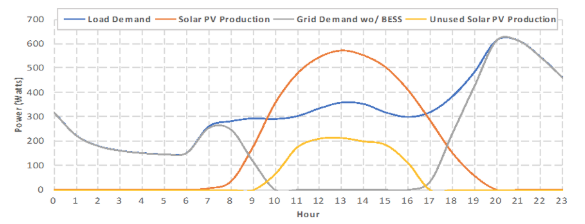
\includegraphics[width=1\textwidth]{./Images/grafico_intro}
\caption{Average household production and consumption in Madeira}
\label{fig:graph_intro}
\end{figure}

As it can be observed in \Cref{fig:graph_intro}, for the average household in Madeira, the production of solar energy is higher when the consumption is lower. Indeed, the peak consumption usually happens between 7 PM and 9 PM, which is the periods of highest domestic demand. Consequently, in self-consumption only scenarios, there is usually a considerable waste of renewable energy. 


This is the issue that will be addressed by the first pilot of \ac{SMILE}, which is targeted at both domestic and commercial \acp{UPAC}. The goal here is to equip these installations with BESS and specialized \acp{BMS} to maximize the self--consumption of those installations.


\section{Power Share}
The \ac{PS} project has been designed as a future business model for the pilot of \ac{SMILE} describe above, therefore, it assumes a scenario where several solar prosumers are equipped with a \ac{BESS}.
The main goal of this project is developing an end-user application for \ac{ET} that uses blockchain as a payment method and contemporarily provides \ac{EF} through a low-cost and easy to use the system. It is designed to be inclusive, that is to say, it does not target only prosumers but also consumers. By combining \ac{ET} with \ac{EF} we aim to:

\begin{itemize}
\item Foster learning and raise awareness about people energy use;
\item Allow prosumers to further benefit from their surplus energy and foster them to engage in \ac{ET} toward the common good;
\item Increase the share of RES in the energy mix by allowing consumers in need of energy to buy local, green energy from their neighbors. Through \ac{PS} they can have control over price and source of their power.
\end{itemize}


The application will be field-tested in 9 households in Funchal (Madeira), with the support of the research team from the \ac{M--ITI} working on SMILE, whose members helped with participants recruitment and the installation of smart meters and communication infrastructure in each household.
In this respect, it should be pointed out that all transactions carried out through the app will be simulated by the server. This is due to the fact that all prosumers participating in the field-test installed their \ac{PV} power system after 2014, therefore are not allowed to inject the surplus energy to the grid.



Such limitation represents the big potential of a system like \ac{PS}. Indeed, if results from the field-test show that the local community is prone to adopt \ac{ETS}, it could become a viable solution for the local \ac{DSO} to manage and distribute an increased amount of \acp{DER}, while keeping the grid stable. For example, by leveraging blockchain smart contracts, \ac{PS} could enable prosumers to sell stored energy when the market most needs it, thus helping to reduce strain across the grid and make it more efficient for all.
It is opinion of the author that testing this virtual, local microgrid represents a first step towards the development of a smart grid -  “an electricity network that can intelligently integrate the actions of all users connected to it - generators, consumers and those that do both - in order to efficiently deliver sustainable, economic and secure electricity supplies” \cite{OverviewSmartGrid} - in Madeira Island.


In this respect, the field-test of \ac{PS} has a twofold goal:

\begin{itemize}
    \item On the one hand, it is meant to assess users acceptance of \ac{ET} in Madeira Island in order to understand if it could be a viable future business model  for one of the solutions developed in the scope of the SMILE project;
\item On the other hand, it aims to evaluate users understanding  and attitudes toward adoption of blockchain as  payment method.
\end{itemize}


At the time of this writing, the application field-test is ongoing. Since it will end after the deadline for the submission of this document, results from the semi-structured interviews about users acceptance of the system won’t be included in the present work. Nevertheless, users interactions with the app are being monitored through Fabric, a platform for developers made for that purpose. Preliminary results from the analysis of three-weeks data are provided in \cref{chap:evaluation}.

The present document is structured as follow: \Cref{chap:back} provides a review of the work done so far on both \ac{EFS} and \ac{ET} areas, analyzing research and commercial projects. \Cref{chap:implement} presents the architecture of the solution proposed here, describing the rationale behind it, as well as front- and back-end design and implementation stages.
\cref{chap:evaluation} focuses on project evaluation providing some preliminary results. \Cref{chap:conclusions} presents results, limitations and future work.



% If Printing on DOUBLE SIDED pages, the second page should be white.
% Otherwise, comment the following command:
\cleardoublepage
%
%Chapter 2
% #############################################################################
% This is Chapter 2
% !TEX root = ../main.tex
% #############################################################################
% Change the Name of the Chapter i the following line
\fancychapter{Related work and Theoretical Background}
\cleardoublepage
% The following line allows to ref this chapter
\label{chap:back}

This chapter presents some background and related work. The chapter is divided into two main sections: \ref{sefs} \nameref{sefs} and \ref{sets} \nameref{sets}. Section \ref{sefs}  provides some literature review about \acp{EFS}, with a focus on the most effective methodologies for designing \ac{EFS}, followed by a review of some research and commercial projects. Section \ref{sets} presents instead some important concepts around blockchain technology, the rationale behind the use blockchain in the energy sector, and some existing energy trading research and commercial projects that leverage blockchain technology.


% #############################################################################
\section{Eco Feedback Systems} \label{sefs}

As mentioned before, Eco-Feedback is defined as a technology that "provides feedback on individual or group behaviors with a goal of reducing environmental impact" \cite{Froehlich2010}. Its effectiveness has been demonstrated by over 40 years of research in multiple fields, nevertheless, designing an effective \ac{EFS} is everything but simple. Indeed, it requires a deep understanding of people latent motivations for sustainable behavior.


In the following pages, a brief (and likely not comprehensive) review of the main aspects to consider when designing an \ac{EFS} is presented.


\subsection{Models of pro-environmental behaviour}

Understanding the motivations that lead people to act environmentally is a prerequisite when talking about \acp{EFS}. According with literature on \ac{EF}, the two main models of human behavior to consider in this case are: Rational Choice Model and Norm-activation model \cite{Froehlich2010}.


The Rational Choice Model assumes that human behavior is, like in game theory, based on the evaluation of expected utility. Basically, according with this model, people do things only if the result of their actions brings some reward. This reward may be monetary or not, like comfort, convenience, etc.


The second model implies that moral or personal norms are direct determinants of social behavior, in other words, if a person is aware of the negative impact of his/her behavior, he/she will feel the moral obligation to modify such behavior.


Selecting one model or the other depends on the user type we are designing for and, consequently, it strongly influences the type of feedback information to be presented. For example, a design based on the rational choice model should show savings in the electricity bill, while presenting the impact of the user behaviors on the Amazon forest would be more consistent with a design based on the norm-activation model.

\subsection{Forms and feedback techniques}

\acp{EFS} are learning tools, they provide users with information about the impact of their behaviour in order to trigger a learning process, which should lead them to reconsider their daily needs and, ultimately, to use energy in a more ecological fashion \cite{DesigningFeedback}.


Control over the feedback, its frequency and the information detail are some of the main aspects influencing such learning process. From this perspective, \cite{Darby2006, DesigningFeedback} identified five main forms of feedback, which vary for the degrees of immediacy and control by the energy user:

\begin{itemize}
    \item Direct feedback: available on demand (the user receives the feedback at any time he/she asks for it). This kind of feedback seems to be the most effective (savings have been shown in the region of 5\%-15\%);
    \item Indirect feedback: it consists in raw data processed by the utility and sent to users. Indirect feedback involves a process of learning by reading and reflecting. Savings have been shown in the region of 0\%-10\%;
    \item Inadvertent feedback: learning by association (e.g. associate the use of an appliance to a higher peak on consumption);
    \item Utility-controlled feedback: personalized feedback regarding consumers’ routines and habits;
    \item  Energy-Audits: usually undertaken by a surveyor, they provide a baseline on the “energy-capital” of a building.
\end{itemize}

Having a picture of the main models of pro-environmental behavior, as well as knowing the possible forms of feedback is not enough to explain the complexity behind the design of an \ac{EFS}. The literature suggests also the following set of techniques and motivation strategies that should be taken into account.


\begin{enumerate}
    \item \textbf{Information:} as a rule of thumb, the better the information is (i.e. easy to understand, trusted, relevant for the user, etc.), the bigger the chance that people will act in an environmentally friendly way. According with Froehlich et al. \cite{Froehlich2010}, to be effective, the information should be presented in an attractive and memorable way, and provided at the time and place the information is more relevant for the user.
    
A lot of studies have been carried out in order to identify the best form for presenting feedback data \cite{Fitzpatrick2009, Giulio2009, Petkov2011, Strengers2011}. First of all, in terms of metrics, it should be pointed out that different individuals have different attitudes and understanding towards energy use. Thus, the metric used for providing feedback should be consistent with the target audience motivations. For instance, it seems that people find environmental impact (CO2 emissions) quite hard to interpret, at least if they are not highly environmentally concerned \cite{Fitzpatrick2009}. For this reason, it is a good strategy to represent such “less-common” units through visual analogies \cite{Strengers2011}, as it is the case of EnergyWiz \cite{Petkov2011} . Here \Cref{fig:energywiz}, CO2 is illustrated as the number of trees necessary to absorb the emitted carbon dioxide due to user consumption. Another interesting aspects to consider is that, despite people do really like the possibility to access a detailed analysis of their energy usage, a certain lack of https://www.overleaf.com/project/5b998b93002024156076f5f0accuracy is not considered a big issue by the most of the users \cite{Fitzpatrick2009}. Indeed, people are usually more interested in seeing their patterns, instead of minor details that could be accessed at ad hoc times, on demand. Thus, as suggested by Jacucci et al. \cite{Giulio2009}, the general rule when designing an \ac{EFS} is to keep it simple; the information should be self-explanatory and must not be presented all at once, but on successive levels of detail, to avoid information overload.

\begin{figure}[h]
\centering
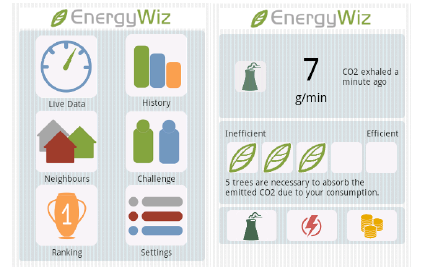
\includegraphics[width=0.7\textwidth]{./Images/energywiz}
\caption{Energy Wiz: main menu and live data}
\label{fig:energywiz}
\end{figure}

\item \textbf{Comparison:} 
comparison has been demonstrated to be an effective strategy in fostering behavioral change. In general terms, there are two types of comparisons: self-comparison (comparison between one’s current and past data) and social (comparing one’s data to that of other households). Social comparison fosters competition \cite{Froehlich2010} and could then strongly motivate behavior change. According with \cite{Petkov2011}, three main types of social comparative feedback can be identified:
\begin{itemize}
    \item Normative: it consists in the comparison between the user’s data and a reference value / an averaged performance. The main issue with normative comparison is that users are prone to be suspicious about the validity of the group they are assigned to \cite{Darby2006,Fitzpatrick2009}. 
    \item  One-on-one: as the name suggests, it consists in the comparison between two individuals, and has been demonstrated to be more effective if the two individuals are closely related (e.g. friends) or share the same beliefs and opinions.
    \item Comparison by ranking consists of comparing groups which are ordered depending on their performance. This type of comparison helps to foster a sense  of competitions between individuals or groups that are not closely related.
    
    In \cite{Petkov2011} the effectiveness of self-comparison, normative comparison, one-on-one comparison and ranking is tested. To this aim, the authors developed the EnergyWiz application, which combines the above-mentioned feedback types , is integrated with Facebook, and allows users to share their consumption or challenge other people to save energy. 

\end{itemize}

\item \textbf{Goal Setting:}
goal setting is a powerful source of motivation and, when combined with feedback, is particularly effective in stimulating environmentally responsible behaviors \cite{Froehlich2010}. The Energy Life application \cite{Giulio2009}(\cref{fig:energylife}) largely relies on such game-like rational. Main aim of this project is to increase people knowledge about the impact of their consumption patterns, and does so by combining awareness tips and consumption feedback. Energy Life presents the users with a series of goals, as well as tips to reach them, tailored on their own consumption habits. Also the above-mentioned EnergyWiz app \cite{Petkov2011} presents a similar feature. In order to increase savings and users engagement, EnergyWiz allows users to challenge a Facebook friend of theirs by proposing a energy saving competition. Results from the interviews with the users revealed that this feature was their favourite. 

\begin{figure}[h]
\centering
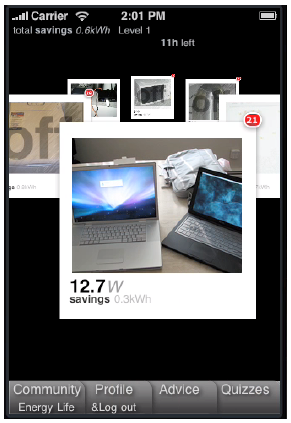
\includegraphics[width=0.3\textwidth]{./Images/energylife}
\caption{Energy Life Menu}
\label{fig:energylife}
\end{figure}

\item \textbf{Commitment:}
it has been widely demonstrated that when a person commits him/herself to behave in a specific way, the probability that s/he will pursue that behavior increases \cite{Froehlich2010}. In the field of Eco-Feedback, for instance, public commitment could lead to energy savings around 20\% \cite{CommitmentandVoluntaryEnergyConservation}

\item \textbf{Incentive / Disincentives and Rewards / Penalties:}
according with Froehlich et al. \cite{Froehlich2010} also incentives/disincentives and rewards/penalties can be used as motivation techniques when designing an \ac{EFS}. Specifically, the former two are antecedent motivation techniques, since they come before a behavior, while rewards and penalties are consequence motivation techniques, which should be used to provide users with some insights into what behaviors they should pursue and what to avoid \cite{Froehlich2010}. Indeed, as pointed out in \cite{Giulio2009}, feedback should not only punish or discourage bad habits, but also encourage good ones.

\item \textbf{Frequency and temporal granularity:}
researchers agree that feedback has a positive impact on behavior change. However, it is a way more efficient if given frequently \cite{Feedbackonhouseholdelectricityconsumption:atoolforsavingenergy?}. The real-time feedback is the most effective one \cite{Froehlich2010} since it helps the users making an immediate connection between an action and its impact, thus making the information more relevant for the user \cite{Fitzpatrick2009}. At the same time, the historical detailing of energy consumption is a highly appreciated feature \cite{Giulio2009, Petkov2011} and really helps increasing users awareness about their energy patterns \cite{Fitzpatrick2009}.

\item \textbf{Media/device:}
some of the studies \cite{Fitzpatrick2009, Froehlich2010, Pereira2013} also highlight the importance of the mobility aspect. Households usually value the opportunity to access the feedback and check their energy status via mobile devices.

\end{enumerate}

\subsection{Research studies on EFS}

\textbf{\ac{SINAIS} project}


Over 40 years of research on \ac{EF} has yielded many insights into designing and effective \ac{EFS}, nevertheless, there are still some interesting research questions to answer and technological solutions that could be used to improve the effectiveness of such systems. This section presents some of the research studies done in recent years for the purpose of \ac{SINAIS}, a research project developed by researchers from the Madeira Interactive Technologies Institute, where part of the present work has been carried out.


\ac{SINAIS} is a long-term real-world research project that combines \ac{NILM}, social networking and context awareness to understand and motivate people to reduce their energy consumption, while trying to fill the lack of research studies that assess the long-term effects of \ac{EFT} \cite{Pereira2012}.


\ac{NILM} - which consists in a system that separates data collected from a single point of measurement into appliance-specific energy consumption data, by using signal processing, and statistical learning - acquires data from sensors that measure current and voltage and then converts them into traditional power metrics. Every time that a significant change in the signal is detected, it is flagged as an event for further processing (i.e. power event are classified through machine learning algorithms). At the end of this process, it is possible to estimate the energy consumption by appliance. One of the main requirement for the study was to develop a low-cost \ac{NILM} solution, which could be deployed in dozens of houses while keeping the installation and monitoring costs low.


 In terms of hardware components, the custom end-to-end \ac{NILM} home energy monitor system developed for the purpose of \ac{SINAIS} consists of a simple netbook. Current and voltage is sampled by using the netbook’s built-in Analog to Digital Converter of the audio input. Feedback on energy consumption is provided through display and speakers, and the communication over the Internet is performed using the Wi-Fi card. In addition, in order to monitor users’ engagement with the system, microphone and built-in camera were used to sense human-activities.  From the software side, data is read from the sensors using Java sound API, and then stored in a centralized repository that uses a web-based hosting service to keep all database files synchronized in one place as long as there was internet connection available. The database is updated every 20 minutes by the meters. The server has many RESTful web-services to access data aggregated in several ways. \Cref{fig:sinais}  illustrates the SINAIS NILM software architecture.
 
 \begin{figure}[h]
\centering
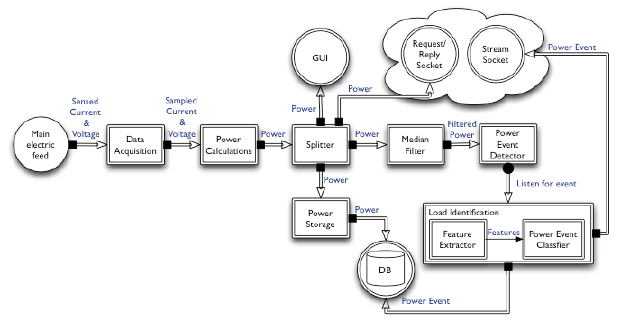
\includegraphics[width=0.8\textwidth]{./Images/sinais}
\caption{\ac{SINAIS} architecture}
\label{fig:sinais}
\end{figure}


As stated above, despite the large amount of research in the area of Eco-Feedback, almost all studies are limited to short periods of time, thus resulting in a reduced knowledge of the effectiveness of \ac{EFS} in the long-term. For this reason, as part of \ac{SINAIS}, the \ac{NILM} system previously described was used in a one-year study, precisely aimed at deepening our understanding of long-term effectiveness of \ac{EF} \cite{Pereira2013}. A total of 12 families used the system for 52 weeks. Results show that after about 4 weeks users stopped paying attention to the system, suggesting that \ac{EFS} are not particularly effective in keeping users engaged over time. To test this hypothesis, a new interface (\cref{fig:efs1}) was introduced (week 8), resulting in an immediate increase in the user interaction. Nevertheless, once the novelty effect has passed (three weeks after the introduction of the new \ac{UI}), the number of interactions dropped again. The same phenomenon was observed around week 20 and 42, when the research team conducted some interviews which temporarily raised participants awareness about the system.
At the end of the study, the interactions decrease was of 90\%. When asked about this decrease of interest in the \ac{EFS}, users justified it due to lack of time as well as as result of a more accurate picture of their consumption patterns


\begin{figure}[h]
\centering
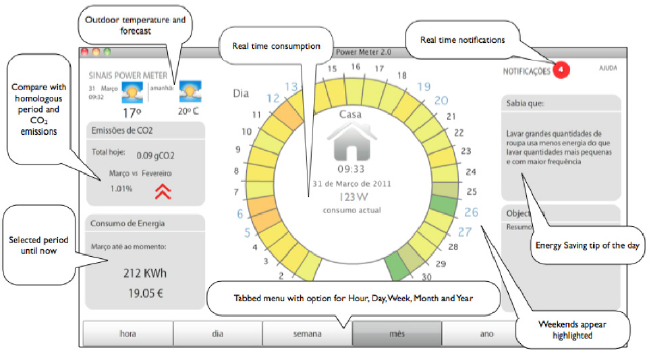
\includegraphics[width=0.8\textwidth]{./Images/efs1}
\caption{The\ac{SINAIS} \ac{EFS} layout}
\label{fig:efs1}
\end{figure}


In order to understand what could lead users to retain attention over time, families’ motivations for sustainable behaviors were further investigated in a two-years study \cite{Barreto2014}.


Interestingly, after interviews with the 15 families that participated in the study, it was found that motivations for sustainable behavior may not be rooted only on individuals’ environmental concerns and/or need for expense management. Other motivations emerged from the study, and not reported in literature, are:

\begin{enumerate}
    \item parenting: parents’ self-perceived responsibility of their role as parents may lead them at engaging with eco-friendly behaviors;
    \item self and family identity: sustainable behaviors as an expression of a pro-environmental identity;
    \item sense of control: families reported a need to know more about their consumption pattern as well as its impact. Accessing this information provided them with a sense of control on their actions.
\end{enumerate}

Another aspect that deeply influence people willingness to adopt more sustainable behaviours  is related to families routines. Indeed, it was found that families (especially those with young children) are less committed to change their consumption habits if they feel it could compromise or affect the completion of the household’s daily tasks. 


Last but not least, household size and children age (if any) have been found to be key variables in understanding families’ latent motivations for pro-environmental behaviors, suggesting that different family types have different motivations. For instance, routine and parenting seemed to be the main motivations of families with young children, while motivations of parents with older children (older than 10 years old) are mainly rooted in short-term goals, like the need for expense management. To sum up, results from this last study suggested that an EFS able to foster long-lasting behavioral changes must go beyond individual ideals of pro-environmental behavior and address basic family needs.


\subsection{Commercial projects}

Not only the research community is involved in the area of \ac{EF}. Many \acp{EFS} are available on the market. Some of the noteworthy products are presented below.



\textbf{Open Energy Monitor} \cite{HomeEnergy}: \ac{OEM} system monitors in real time the energy consumption/production (solar or electrical) and provides feedback also regarding historic data and energy cost. It is fully open-source (hardware and software). The hardware is Raspberry Pi and Arduino based and works over wifi. Market price ranges from about 155£ (without sensors) to 189.80£   for the solution including all sensors \url{https://shop.openenergymonitor.com/emonPi-3}.


\textbf{Sense} \cite{sense}: consists of a small computer, connected to the electrical panel, that monitors both solar production and energy consumption (overall as well as appliances breakdown). Through an application, it provides feedback about: 
\begin{enumerate}
    \item real-time consumption / production; 
    \item historical energy trends (available by day, week, month and device) and; 
    \item usage statistics for individual appliances.
\end{enumerate}

 This system requires a few weeks of training in order to recognize the devices, and does so through advanced machine learning algorithms.The price is higher compared to \ac{OEM} and ranges from 299\$ (for the system monitoring only power use) to 349\$ for “Sense Solar”. Also, the fidelity of the results decreases when the network of sense users is small, because machine learning algorithms will produce less reliable results.



\textbf{Efergy} \cite{efergy}:
claims 25\% savings in the electricity bill (more than the 10-15\% reported in \ac{EFS} literature), but no data or studies to prove that were found. Their Online Energy Monitor Home \& Solar consists of a real-time energy monitoring system that can be integrated with a set of smart-plugs and a mobile app to monitor and control the single appliances. This system is powerful but not easy to install and also quite intrusive, since it requires installing a socket for each appliances to control. As an example, a complete kit with five meters has a cost of 219,60€\footnote{This value was consulted in September 2018: \url{https://efergy.com/store/en/online-energy-monitors/18-online-multi-circuit-energy-monitoring-kit.html\#/35-number_of_circuits_to_monitor-5_x_1ph_circuit}}, and extra meters are about 54,90€\footnote{This value was consulted in September 2018: \url{https://efergy.com/store/en/accessories/22-submetering-kit-stxtra.html\#/28-select_your_power_supply-3_phase_up_to_90a_phase}}.



\textbf{Neurio} \cite{neurio}: is another monitoring system that can be easily installed within the home’s load panel and provides feedback on both production and consumption.



\textbf{Energeno}: developed several models of energy monitoring systems. Despite these systems were pretty well-known and have been analyzed in several research studies, Energeno has ceased trading.


\subsection{Conclusions}

The projects listed above combine many \ac{EF} techniques like real-time feedback, which is one of the most effective \cite{Froehlich2010}. The \ac{SINAIS} project introduced machine learning algorithms to identify the source of energy consumption, however, despite users appreciated the opportunity to better understand what appliances consume more \cite{Pereira2013}, after one year deployment, the decrease of energy usage was not significant. This result support the hypothesis that \acp{EFS} are not effective in long term because, as suggested by results from \ac{SINAIS}, after a while people lose interest in the system which become “ just another electric device” \cite{Pereira2013}. Another important lesson learned is that \acp{EFS} must be designed to adapt to different users (and, consequently, different behaviours, needs and interests). For the same reason, as demonstrated in several of the studies reviewed, the mobility aspect is extremely important. Users want indeed to access their data quickly and from virtually everywhere; that’s why commercial \acp{EFS} like Sense and Efergy provide users also with a mobile application. Ultimately, it is important to point out two main weaknesses of \acp{EFS}. On the one hand, the cost. \acp{EFS} available on the market are quite expensive and this could explain their low adoption rate. On the other hand, the fact that their effectiveness decrease in long term \cite{Pereira2013}, which suggests the need of thinking about solutions that could keep users engaged and interested in the system over time. 



% #############################################################################
\section{Energy Trading Systems using blockchain} \label{sets}
\subsection{Blockchain}

Blockchain is a technology for peer-to-peer platforms that has a decentralized storage to record all transaction data. This technology came into the public in 2008  when a publication by Satoshi Nakamoto (a pseudonym for the creators)  launched Bitcoin, describing it as a \ac{P2P} electronic cash system that enables online payments to be transferred directly without an intermediary \cite{bitcoin}. Bitcoin is one application of the blockchain concept, the first and the most known one:  “Blockchain is to Bitcoin, what the internet is to email. A big electronic system, on top of which you can build applications. Currency is just one.” - Sally Davies, FT Technology Reporter \cite{Howbitcoinanditsblockchainwork}. However, this technology has a great potential in many sectors, not only in the financial one.


First, we will introduce the main concepts before explaining how they will be applied in this project. The blockchain concept relies on the decentralization idea. A decentralized storage and decentralized business without need of a trusted third party are the base of this technology. Short time ago, all money transactions were executed by trusted third parties like banks and governments, resulting in extra costs for the customers. The role of those entities is to authenticate both participants of the transaction (the emissary and the receptor) and keep the record as a confirmation of the transaction. In this digital world, it is even more important to securely store the record of the transactions in order to prevent any malicious activities. 



\subsubsection{Overview}


Electronic coins are chains of digital signatures and a transfer is done signing a hash of a previous transaction and the public key of the next owner and finally adding these to the end of the chain \cite{bitcoin}. The main problem here is a guarantee that the coin is not double-spended \footnote{the ​double spending problem ​is a potential flaw in a cryptocurrency or other digital cash scheme whereby the same single digital token can be spent more than once, and this is possible because a digital token consists of a digital file that can be duplicated or falsified.Chohan, Usman, The Double Spending Problem and Cryptocurrencies (December 19, 2017). Available at SSRN: \url{https://ssrn.com/abstract=3090174} or url{http://dx.doi.org/10.2139/ssrn.3090174}}. Usually the double-spend problem is solved by a centralized trusted authority that is responsible to guarantee that the rules are not broken. This is a single point of failure approach, \textit{technically speaking} this means that the centralized authority has all data (electronic coin representation) in the same place (or machine) and in case of this data be compromised, all the system will be compromised too, in the trusting level, the users of a system with this approach are required to trust in the authority and if that authority is a malefactor all the user data will be in risk.  The blockchain technology eliminates the need for intermediaries, validating the transactions in a decentralized way. 


The transactions are carried out between peers who can be providers, consumers or both. The data that contains all the relevant information about the transaction is stored on a distributed ledger and all peers store the block of data locally. A distributed ledger is a distributed database that records, shares and synchronizes transactions in different locations. It is efficient, resilient and reliable. 


Ideally, all of the transactions have a smart contract behind. Smart contracts define the rules related to the transaction, like a transactions protocol that executes the terms of a contract \cite{SmartContracts}. \cref{fig:bc} demonstrates the idea of transaction validation.



 \begin{figure}[h]
\centering
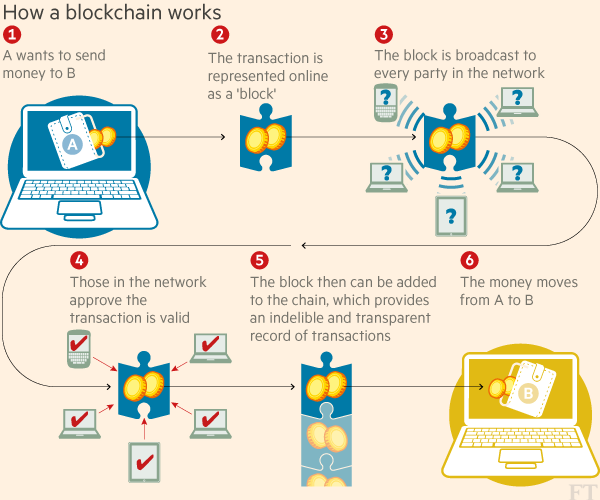
\includegraphics[width=0.8\textwidth]{./Images/ft}
\caption{Illustration about transaction validations workflow in blockchain}
\label{fig:bc}
\end{figure}


Each transaction is encrypted and distributed to individual computers and each member of the network stores the data locally. Each block is verified using hash algorithms and associated with a hash that is unique and is related to the information on the blockchain. If the information on the block is changed after the transaction, the peers cannot verify the block because the correct hash is not produced anymore, and the block is discarded.



The continuous verification is called mining and is performed by the members of the network. The mining is necessary to ensure that everyone agrees on the order of the transactions. Each block is like a package of transactions and is associated with a timestamp, a nonce and a reference to a previous block (i.e. hash of the previous block) \cite{bitcoin}. All these blocks connected form a blockchain that is constantly growing and represents the state of the ledger.


To establish that consensus, both proof-of-work and proof-of-stake are used.
In the \textbf{proof-of-work} approach, each block is verified by a large group of peers before storage using algorithms that associate a unique hash (ordinary or cryptographic) to the block. The verifying task is very complex because it is necessary to find a hash that corresponds to the block content. The block cannot be changed without re-doing the work and if a new block is added to the chain after this one, all blocks after this need to also re-do the work \cite{bitcoin}. This process requires a lot of energy. If a block content is verified by the majority of peers it can be added to the blockchain, otherwise it is discarded. This majority decision is represented by the longest chain, which means the one with the greatest proof-of-work effort invested \cite{bitcoin}. 


\textbf{Proof-of-stake} approach is simpler than the proof-of-work approach because it requires that users prove ownership of their own share (stake). So, if a user owns 10\% of total data he just needs to be mining 10\%. This reduces the complexity of the task and is less expensive in terms of costs and energy consumption \cite{etherium}.
Summarizing, the steps performed in a blockchain network are \cite{bitcoin}: 

\begin{enumerate}
    \item New transactions are broadcasted to all nodes. 
    \item Each node collects new transactions into a block. 
    \item Each node works on finding a difficult proof-of-work for its block. 
    \item When a node finds a proof-of-work, it broadcasts the block to all nodes. 
    \item Nodes accept the block only if all transactions in it are valid and not already spent. 
    \item Nodes express their acceptance of the block by working on creating the next block in the chain, using the hash of the accepted block as the previous hash.
\end{enumerate}


The main disadvantage of the blockchain technology is its performance. The blockchain technology implies heavy calculations, the mining process explained above, to generate and verify the signature of each block. Due to its decentralized nature, an extra effort is necessary to ensure a consensus exists in the network. Consequently, the total amount of computation that a blockchain requires per node in the network is very expensive in relation to a centralized database. The fact that blockchain is a recent technology can be seen as disadvantageous because it is necessary for a new technology to have existed for a longer period of time in order to increase cultural adoption and trustworthiness. The large energy consumption in Bitcoin blockchain is a very big problem, but this problem was reduced with the emergence of the Etherium approach which uses three times less energy than Bitcoin because it uses the proof-of-stake method to verify transactions.


The advantages of the blockchain technology are bigger than the disadvantages. The main advantages include lower costs, faster processes and greater flexibility because no more third parties are needed and no central point of failure exists once the storage and communication are fully decentralized. All the time and money spent to prevent tampering in centralized databases is not necessary anymore, because in blockchain the storage is not centralized. Other significant advantages are the control that users can have over all the information and transactions, the consistency and availability of the data, the trustworthy process of each transaction, the faster transactions and the lower costs per transaction.


\subsubsection{Integration in the energy sector}

Traditionally, the Electrical Power Systems are controlled via a top-down approach where central authorities are responsible to manage the energy distribution in the grid. Lately, new decentralized approaches are being investigated in order to create a full transparency and to allow micro producers and consumers to reap the full economic benefit of the energy sharing system without the participation of central authorities. The Blockchain could be applied to the energy market providing a secure decentralized network to share energy \cite{Hasse2016}. There is an especially high potential for energy trading, automation of processes and new business models \cite{UseCasesforBlockchainTechnologyinEnergyCommodityTrading}. Another novel application is the use of cryptocurrencies in the payment system. The storage of energy data can also be re-designed to work over blockchain technology with smart contracts and verification of transactions ensuring the integrity of the data and trust between the grid participants \cite{ETHome:Opensourceblockchainbasedenergycommunitycontroller}. For example, in a smart grid, a producer who has more energy than he needs can automatically sell the excess energy via a smart contract to neighbours who want to buy energy. This example can be done in the reverse order, i.e. consumers can automatically buy energy from other producers.


 The concept of a blockchain based distributed controller for the efficient share of \acp{ESS}  has been proved showing that the concept is applicable, scalable and economically feasible \cite{ETHome:Opensourceblockchainbasedenergycommunitycontroller}. Also, secure and privacy-friendly protocols were designed for trading and billing in Smart Grids \cite{SecureandPrivacy-FriendlyLocalElectricityTradingandBillinginSmartGrid} and can be applicable. 

\subsubsection{IOTA and the Tangle}


Since increasing the consumption of renewable energy is one of the main goals of the present work, it would have been inconsistent to not use an efficient blockchain platform. After some research, the IOTA distribution ledger technology has been identified as the most suitable solution for that purpose. IOTA is an open-source distributed ledger, which differs from blockchain concepts like Bitcoin or Ethereum, since it uses “The Tangle”,a \ac{DAG} characterized by high scalability and low resource requirements. The Tangle eliminates one of the biggest drawbacks of blockchain, that is to say, it removes fees \cite{WhatisIOTA}. Since IOTA cryptocurrency is open source and blockless, users can make transactions on the network for free. In addition, this cryptocurrency is very well rated in terms of market capital (10th place, at the time of this writing \url{https://coinmarketcap.com/}).  The absence of fees is extremely important, especially when we are talking about micropayments, like in the case of \ac{P2P} energy trading. While in traditional blockchain transactions are grouped into blocks and stored in sequential chains, the Tangle is blockless and no third party are needed.. Individual transactions are interconnected in a \ac{DAG}. For example, let’s take a scenario where A, B, C and D are different nodes of the network, and A wants to communicate with D. In a traditional blockchain network, which is sequential, the transaction between A and D needs to be distributed and validated by both B and C before it gets to D. On the contrary, on the Tangle A, B, C and D are connected in a braid-like fashion, thus, when A needs to communicate with D, it sends the data directly to D while synchronizing (almost) instantaneously B and C. Consequently, the energy spent for the proof-of-work is reduced, since consensus is established only by the participants making transactions instead of miners.


The main idea of the Tangle is that, when a transaction issued by a node arrives, it must approve at least two previous transactions. This way, users who issue a transaction are also contributing to the security of the network \cite{TheTangle}. Steps to issue a transaction are the following \cite{TheTangle}:

\begin{itemize}
    \item Signing the transaction with private keys;
    \item Selecting two “tips” (i.e. unverified transactions) using \ac{MCMC}) algorithm. Then, if they are not conflicting, the node approves them;
    \item Solving a cryptographic puzzle by finding a nonce such that the hash of that nonce concatenated with some data from the approved transaction has a particular form.
\end{itemize}

After a transaction is performed, it is broadcasted in the network and validated by the active members of that network. To keep the state of the network a consensus protocol is used, which decides if a transaction could be safely considered confirmed or not . 

The \cref{fig:tangle} below represents the structure of the Tangle and how the validation process works - green nodes are the verified transactions; red nodes represent transactions in process of verification; grey nodes are the unverified transactions (tips).
Green blocks are indirectly referred by all the grey blocks, thus, for every confirmed transaction there is a path that goes to a tip. Now, the node runs the tip selection algorithm (\ac{MCMC}) N times; the number of times the transaction is selected determines the confirmation level of that transaction. For instance, if a transaction is selected 55 times during 100 runs of the \ac{MCMC} algorithm, that transaction is confirmed with 55\% confidence.



 \begin{figure}[h]
\centering
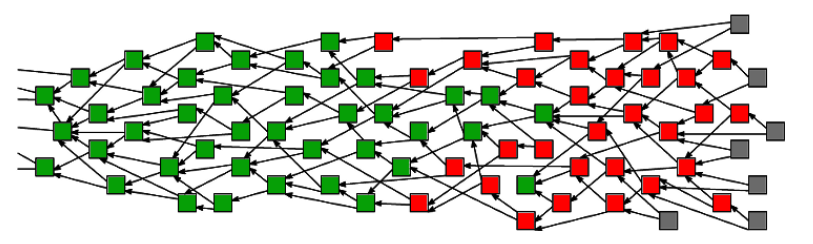
\includegraphics[width=0.8\textwidth]{./Images/tangle}
\caption{The thangle \ac{DAG}}
\label{fig:tangle}
\end{figure}


To sum up, the main features of IOTA are:
\begin{itemize}
    \item Data Transfer through the tangle in a securely and authenticated way.
    \item Masked Messaging: all the exchanged data can be encrypted and authenticated. With \ac{MAM} data is shared by multiple parties and these multiple parties can adjust the frequency and get the broadcast data.
    \item Everything as a service: anything with a chip can be leased in real time.
    \item Scalable ledger.
\end{itemize}


In order to perform transactions on the tangle users need to have a IOTA seed, which consists of a 81, 162 or 243 characters string (only uppercase latin letters and 9’s) and is generated randomly. Through the seed, a user can access his/her IOTA account, thus, the seed is secret and must be securely stored. In addition, to receive payments, the user needs a destination address. This address is generated from the seed and can be public.


Further details about how the Tangle works and how it will be employed in this project are provided in \ref{ii} \nameref{ii}. 


\subsection{Research projects and startups}


At the time of this writing, several projects have been launched with the goal of building a distributed energy system. According with the Event Horizon 2018 Startups report, about 41 startups are developing blockchain-based energy applications (25 of them in Europe), nevertheless, after a quick search, a lot more blockchain startups working in the energy field can be found \cite{EnergyBlockchainStartups}. In this scenario, Etherium seems to be the most used blockchain protocol \cite{STARTUPSWHOISWHO}.



Below, a review of some existing projects is provided. Given the rapid evolution of this sector, such review makes no claim to be comprehensive. In addition, the reader should be warned that ost of the projects here described are under development, thus many details about them are still unknown. 



\textbf{Electron} has been launched by “a team of blockchain, energy and e-trading professionals using decentralized technology to advance the shared infrastructure of the energy markets” \cite{Electron}. In general terms, Electron is a marketplace for energy and flexibility services underpinned by a \ac{DER} asset registry \cite{STARTUPSWHOISWHO}.
Their approach is more collaborative, top-down than peer-to-peer. Electron is looking for a shared infrastructure and collaboration opportunities to change the energy market. One of the main projects they are involved in aims to unlock \ac{DSR} by using blockchain technology \cite{demand-sideresponse}. The goal of this project is creating an incentive for everyone in the market (grid operators and largely energy users); users that reduce their energy consumption on peak periods will receive a payment for that and consequently if the demand is reduced at peak time the electricity prices should lower.



\textbf{Power Ledger} is a decentralized energy trading blockchain based platform that enables residential and commercial businesses connected to the existing distribution network to decide to whom they sell their energy and at what price \cite{STARTUPSWHOISWHO}. Their solution is peer-to-peer and allows direct selling and buying between micro producers and consumers without a third party involved and with payment in real time. The system is based on blockchain but the payments are made with fiat-currency\footnote{is a legal tender that is backed by the sovereign government state that issues it. The
Australian dollar and U.S. dollar is fiat money, as are many other major world currencies. This differs
from money whose value is underpinned by some physical good such as gold or silver (commodity
money).}.



Power Ledger is a dual-token platform: POWR tokens are used to access the platform and can be exchanged for the other token (Sparkz), which is a stable (i.e. pegged to fiat currency) exchangeable frictionless energy trading token Spark must be pre-purchased \cite{powerledgerwhitepaper} and can be then redeemed for fiat currency. \cref{fig:plp2p} represents the \ac{P2P} trading between consumers and prosumers through Power Ledger. 




 \begin{figure}[h]
\centering
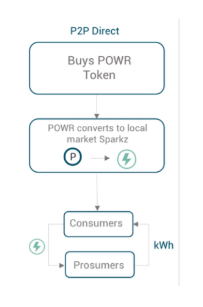
\includegraphics[width=0.3\textwidth]{./Images/plp2p}
\caption{\ac{P2P} trading through Power Ledger}
\label{fig:plp2p}
\end{figure}


To sum up, users must buy POWR tokens to sign in and use the platform. After that, POWR tokens are converted to Sparkz (local market level token), which in turn can be used to perform the frictionless exchanges - that is to say, payments for the transactions are made via local currency, not cryptocurrencies. Power Ledger has adopted a hybrid public and consortium blockchain approach. POWR tokens are generated on the public Ethereum blockchain (proof-of-work algorithm), while for the P2P energy trading a fee-less Ethereum blockchain is used. The next step is migrating all system on a public proof-of-stake blockchain, which would be more sustainable. Specifically, this blockchain is called EcoChain and is still under development.



So far, Power Ledger is one of the most advanced projects in this area, and has been successfully pilot-tested since 2016. The first pilot was indeed a big success; 15 dwellings were connected via blockchain, so to provide them with a secure channel for direct exchange between Sparkz and currencies in real-time, and used distributed ledger technology to facilitate “across the meter” energy trading and manage the \ac{DER} assets without going through an electricity retailer. Power Ledger algorithm is developed to respond in real-time to both network conditions and consumer behavior.   


\textbf{LO3 energy Inc.} is developing blockchain based solutions for the energy market \cite{lo3energy}. Together with \textbf{Transactive Grid}, LO3 designed the first community-powered microgrid: the \textbf{Brooklyn Microgrid} \cite{lo3energy}. Using blockchain, residents with solar panels can sell excess energy to their neighbours in a peer-to-peer transaction.The energy is transmitted by the conventional power grid, and transactions are recorded d and managed using the EXERGY, a blockchain enabled platform with smart contract functionality at its core [source]. Production and consumption data are collected through smart meters and than hashed into the blockchain. Through a mobile app, users can also choose what to do with their excess energy(i.e. storing it into the battery, or selling it to the grid or to the neighbors (figure xx, 4th image).  The Brooklyn Microgrid A \cref{fig:microgrid}, rated 4.9 out of 5 on Google Play an App Store, presents the following main features:

\begin{itemize}
    \item Check out the solar panels locations and suggest new ones;
    \item Check solar panel efficiency and where leftover energy is going;
    \item Energy usage feedback (up to 12 months).
\end{itemize}

\begin{figure}[h]
\centering
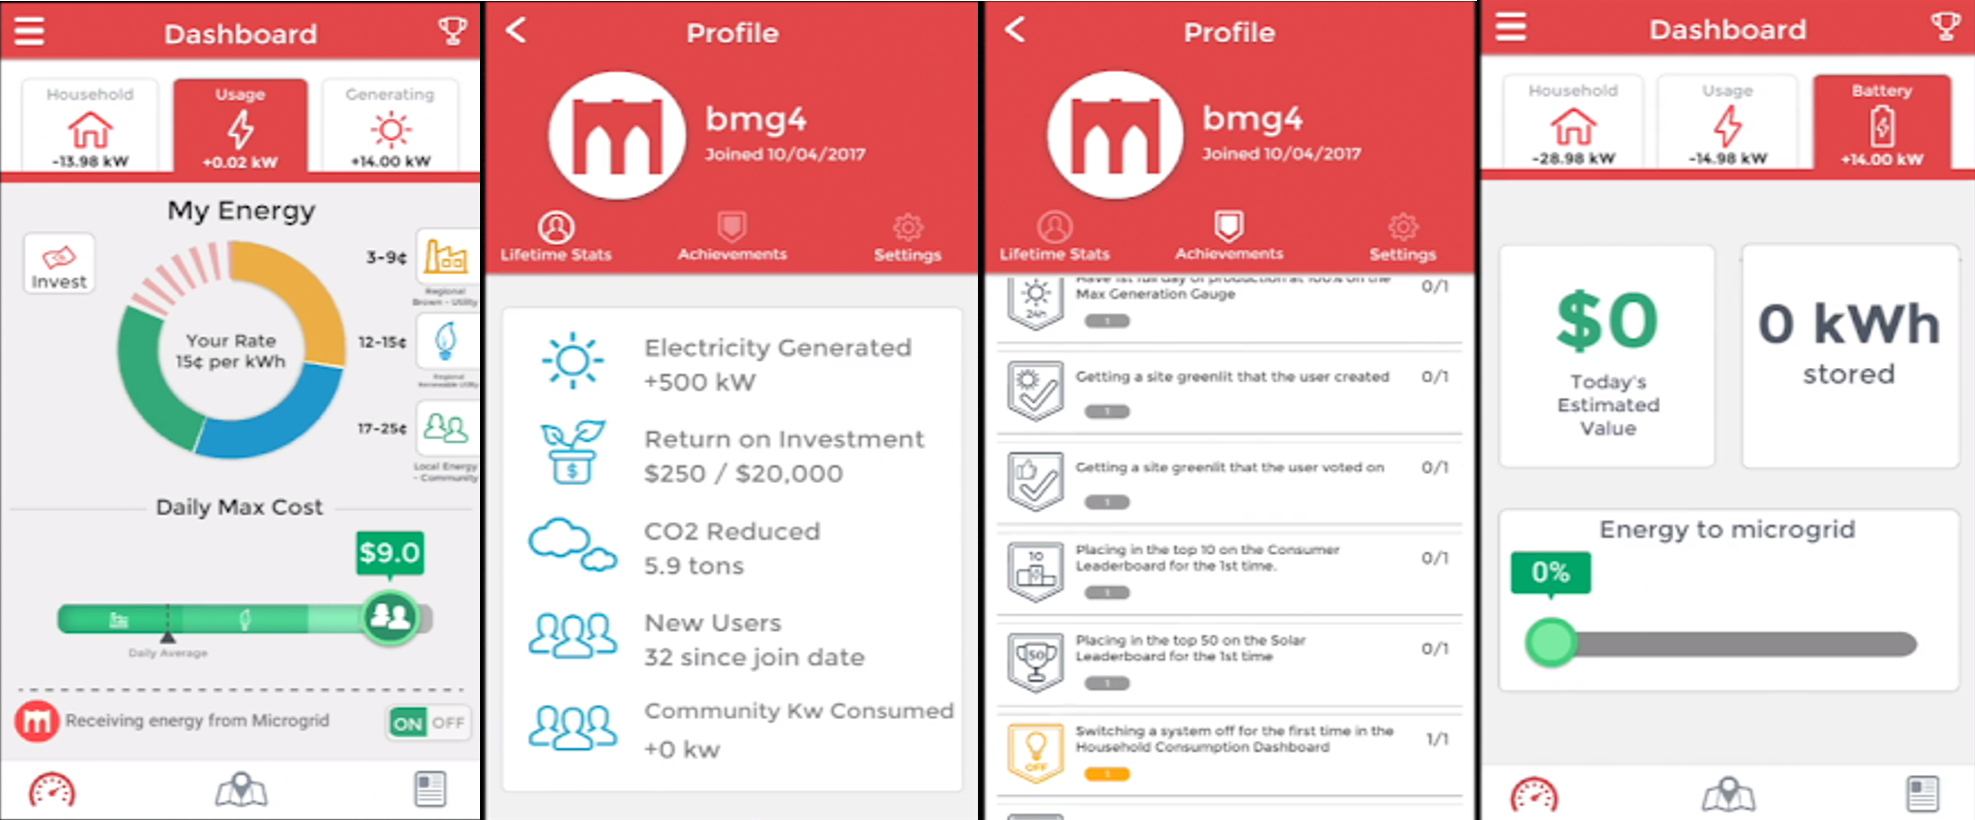
\includegraphics[width=0.9\textwidth]{./Images/microgrid}
\caption{Brooklyn Microgrid application layouts}
\label{fig:microgrid}
\end{figure}

The App works as follows. First of all, users have to set how much are willing to pay for their energy a day (see \cref{fig:microgrid}, 1st image). Such value will consequently determine the source of the energy users are buying. Price of local generated energy is driven by the participants in the local network \cite{vimeo}. In addition, users are provided with the opportunity to turn off their appliances in case of grid overload and get paid for that. Users’ energy stats is provided in the profile page (see \cref{fig:microgrid}, 2nd image). Last but not least, in the achievements sections, users can showcase their reputation as advocates for local energy (see \cref{fig:microgrid}, 3rd image).



\textbf{Omega Grid} consists of a private cyber secure distribution market \cite{STARTUPSWHOISWHO} which uses a blockchain based Financial Energy Resource Management System  to record communications, verify power delivery, and perform transactions. The communication is done via a private mesh network. Omega Grid connects local distribution companies with both prosumers and consumers, providing benefits for all of them \cite{omegagrid}. Like Power Ledgers and Brooklyn microgrid, Omega Grid effectively transmits energy through local grids. Omega Grid uses a energy efficient Proof of Authority consensus model (basically,an optimized Proof of Stake model) that use identity as a form of stake instead of  staking tokens. A group of pre-approved validators is then responsible for staking the identity \cite{poa}. 




\textbf{Leap} is a platform that enables automated trading on energy markets for anyone, including aggregators, utilities and \acp{ISO}.


The platform is based on the \ac{DEX}, which basically consists in an open energy market that allows for fully automated trading of energy resources \cite{leap} (see \cref{fig:leap}). The main goal of Leap is reducing power consumption in peak hours. For this purpose, the \ac{DEX} collects  information about load reduction rewards programs from \acp{ISO} and utilities.


\begin{figure}[h]
\centering
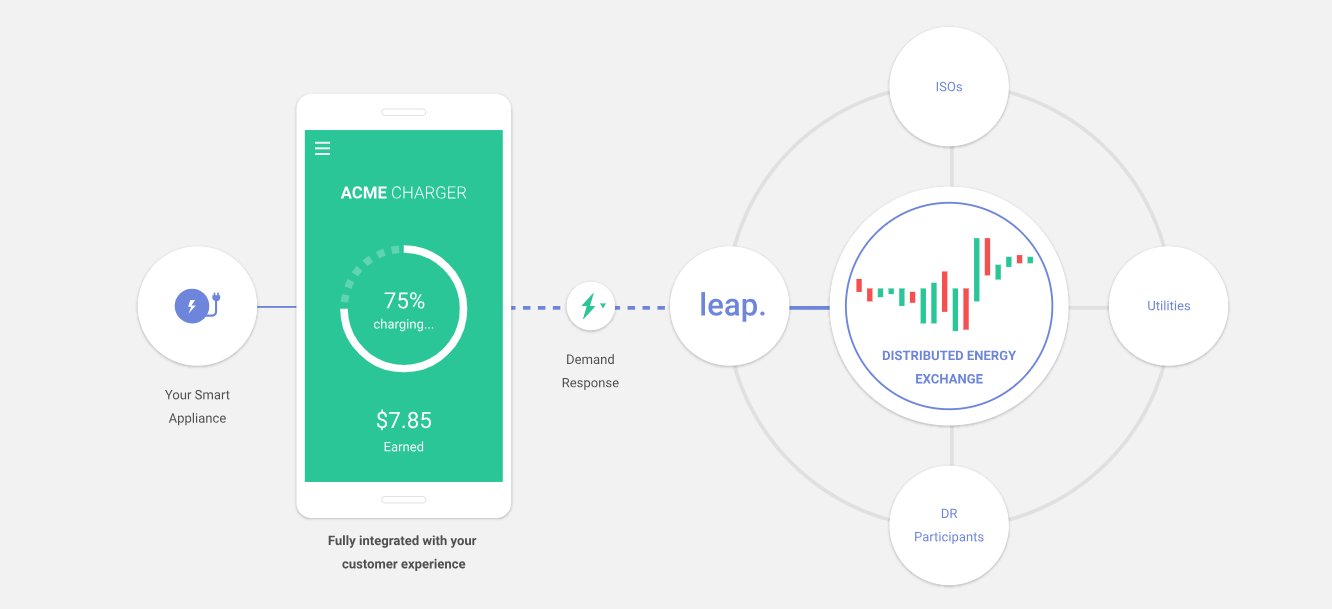
\includegraphics[width=0.8\textwidth]{./Images/leap}
\caption{Leap overview}
\label{fig:leap}
\end{figure}

Then, on the basis of smart contracts, it performs Demand Response control and send meter data back to the \acp{ISO}, who verifies load reduction and remits funds to accordingly. 


\textbf{Grid Singularity}, a startup based in Australia, is developing an open and decentralized energy data exchange platform. Core of the platform is DA3,  a grid management agent that creates a novel market model for the transactive grid, enabling a wide spectrum of energy market related transactions on a single platform layer via blockchain. The platform will be launched in 2019 thus many details are still unknown. Nevertheless, according with an interview to the CEO of Grid Singularity, Ewald Hesse, the platform will work as follows:
\textit{“All data will be recorded in real time on the blockchain, what will make it fully secure and impossible to modify. Once the platform is ready, it will be able to support numerous applications, for example for data analysis and benchmarking, green certificates, smart grid management, investment decision, and energy trade validation. The core product will be invisible for the end users – all that they’ll have to do is download an app that will make their houses single traders in the market”}\cite{gridsingularity}.  	



It’s impossible to list all the projects that are being developed in this field since their number is growing almost on a daily basis. \textbf{Enerchain}, for example, is another blockchain based distributed ledger for energy tradings that use Tendermint\footnote{Tendermint is software for securely and consistently replicating an application on many machines. Works even if up to 1/3 of machines fail in arbitrary ways. Every non-faulty machine sees the same transaction log and computes the same state.See more:\url{https://tendermint.readthedocs.io/en/master/introduction.html}
} technology to guarantee a short block time in order to allow tradings almost in real-time \cite{enerchain}. \textbf{Powerpeers} developed a similar system for P2P energy trading, not based on blockchain yet, that is currently being deployed in Amsterdam \cite{powerpeers}. 



\textbf{\ac{EWF}} is an open-source, scalable, blockchain platform designed for the energy sector. The vision of \ac{EWF} is joining forces to accelerate the transaction to a decentralized, democratized, decarbonized, and resilient energy system. 
	
	
	
Except for Brooklin Microgrid and Grid Singularity, all the projects here described use Ethereum blockchain. Brooklyn Microgrid use Exergy and Grid Singularity uses Energy Web Chain.


The author considers using Etherium as a disadvantage since Ethereum transactions have fees (to “cover” the computing power needed for the proof-of-work). To overcome this issue, Power Ledger, for instance, has developed the EcoChain, a more sustainable blockchain, while Omega Grid uses proof-of-authority consensus model instead of proof-of-work.



Electron, Omega Grid and Power Peers act like an intermediary between energy suppliers and all possible consumers. It is also important to notice that many of the projects and startups described above still need to be deployed and pilot tested. At the time of this writing, only Brooklyn Microgrid, Power Peers and Omega Grid have successfully reach the market. Power Ledger project is well documented and a lot of experiments have been done so far to test the platform. Nevertheless, it has not being launched yet, so it’s hard to evaluate it.



Last but not least, it should be pointed out that only Power Peers, Power Ledger and Brooklyn Microgrid have as main target micro producers and consumers. Focusing on the local community first is a promising strategy, since each community has its own cultural attitudes and motivations toward engaging in P2P energy trading, which should be taken into account when designing such systems. This can be considered an advantage because all the markets have specifics constraints like grid stability, infrastructures architecture and also the cultural differences in the user’s behavior. On the contrary, platforms like Electron, Leap and Omega Grid focus on using blockchain to target energy market problems, like \ac{DSR}, thus opening up space for retailers and electricity companies.   

% If Printing on DOUBLE SIDED pages, the second page should be white.
% Otherwise, comment the following command:
\cleardoublepage
%
%Chapter 3
% #############################################################################
% This is Chapter 3
% !TEX root = ../main.tex
% #############################################################################
% Change the Name of the Chapter i the following line
\fancychapter{System design and implementation}
\cleardoublepage
% The following line allows to ref this chapter
\label{chap:implement}
\section{Introduction} 

The main goal of this work is developing an end-user application for \ac{ET}, that uses blockchain as a payment method and contemporarily provides \ac{EF} through a low-cost and easy to use the system.


Taking into account lessons learned from previous studies in both areas of \ac{EFS} and \ac{P2P} \ac{ET}, the system was designed as a mobile application (developed for Android since it is open source).



Despite all participants in the field study aimed at testing the app are prosumers, \ac{PS} targets also consumers. Therefore, the motto while designing the application was “keep it simple”, that is to say, easy to use and understand for the wider audience possible (including people with a limited knowledge on energy).



\ac{PS} allows automated energy tradings between neighbors. It provides users with the opportunity to set the parameters for buying and/or selling energy, as well as to access and monitor data regarding their energy consumption, production (in case the user is a prosumer), and transactions.



The application is connected with \ac{PS} \ac{ETMS} that is responsible for managing users’ accounts, managing energy demand and offer, and providing data about the users’ overall energy consumption and production. Data are collected through a smart meter, installed in each household participating in the study, which measures production and consumption. The integration of IOTA technology will serve the purpose of carrying out the transactions between neighbors in a decentralized fashion.


\Cref{fig:ps} shows the architecture of the system. The grey arrows represent the regulated electricity network (the power grid*), which is managed by the local \ac{DSO} and is therefore independent of our system. Each household has its own solar PV system and BESS*. When PowerShare \ac{ETMS} find a match between energy demand and offer, it automatically starts the transaction, which is then paid using IOTA node as a service.  

\begin{figure}[h]
\centering
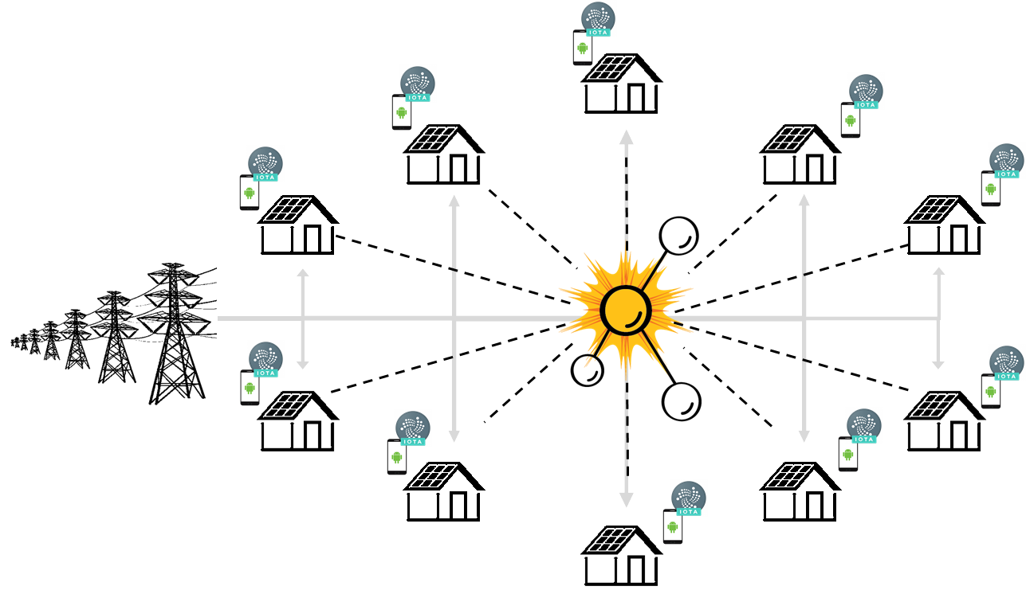
\includegraphics[width=1.0\textwidth]{./Images/ps}
\caption{Power Share system illustration}
\label{fig:ps}
\end{figure}


The following sections provide a detailed description of both front- and back-end of the application, as well as of the integration of IOTA technology. Requirements and constraints that led to the final solution are also presented. 

\section{Power Share Application}


This section describes all the process of design and implementation of the front-end of the \ac{PS} mobile application.



\subsection{Design}


Once the requirements and main goal  were defined, we started designing the front-end of the app.  During an initial brainstorming, we wrote down onto sticky notes a set of aspects (found after reviewing the literature on \ac{EFS} and \ac{ET} and analyzing outcomes of existing projects) related to:

\begin{itemize}
    \item Users needs;
    \item Obstacles to adoption;
    \item Limitations of both systems;
    \item Insights.
\end{itemize}


Then, the stick notes were sorted into groups through an affinity diagram, looking for relationships and patterns. By following this process, the following main sections/features of the app were identified:



\begin{itemize}
    \item \textbf{Home:} showing current consumption and production. Real--time feedback is indeed often defined as a requirement by users of EFS and helps them better understand the link between an action and its effect (e.g. peak consumption after turning on the hair dryer);
    \item \textbf{Settings:}through which the user can define the criteria to buy/sell energy;
    \item {Historical:} provides the user’s consumption/production data over time (which has been found to be one of the most appreciated features by EFS users and, at the same time, provides a set of information that could be of great help in identifying the best criteria to buy/sell energy);
    \item \textbf{Transactions:} showing a list of all transactions made by the user;
    \item \textbf{Ranking:} since social comparison has been proven to an effective leverage to foster behavioral change, this section shows to the user how his consumption of renewable energy compares to the other users.
\end{itemize}


The navigation tree and some basic requirements of \ac{UI}/\ac{UX} were also defined. First of all, the \ac{UI} has to be simple (but not simplistic), user-friendly, clear and appealing. Data provided through the app must be detailed in order to avoid misunderstandings but, contemporarily, limited to the most relevant ones in order to avoid information overload. The “setting” should be designed targeting those users that have a limited knowledge of energy. Also, negative feedback should be avoided.


The resulting wireframes were subjected to a quick heuristic evaluation of layout elements, function, and flow, after which possible bottlenecks were identified and removed. Then, a low-fidelity prototype was realized and tested with a small group of researchers and students from the Madeira Interactive Technologies Institute, all with a limited knowledge of energy.
Participants in the pilot test performed the following tasks:
\begin{enumerate}
    \item Registration of a new account. All participants concluded that task successfully. Since the registration process requires users to input some information about their \ac{PV} installation (in prosumers mode) and contract with the energy supplier, the \ac{UI} included tips to help users filling out the input fields. Nevertheless, some of the participants did not see them immediately, suggesting us to make them more noticeable. 
    \item Modify account settings. Again, all users complete the task, but some of them selected first the “trading settings” feature, suggesting the need to make the purpose of each section more clear by rethinking carefully both labels and icons.
    \item Configure the parameters to buy and sell energy. The main issue here was that users did not understand that there were mandatory (e.g. set a price) and not mandatory fields (e.g. define specific time frame when buying/selling energy). To address this issue sub headers were added as shown in \cref{fig:ps1}.
    \item Check the list of transactions carried out. Some users select “Histórico”. Such a mistake was due to the icons design, which turned out to be misleading.
    \item Check historical production/consumption data. All participants concluded that task successfully and the visualization designed (a stacked bar graph) resulted clear to everyone.
    \item Check current energy usage (Home). All participants concluded that task successfully.
    \item Check your achievements (Rankings). All participants concluded that task successfully.
\end{enumerate}


\begin{figure}[h]
\centering
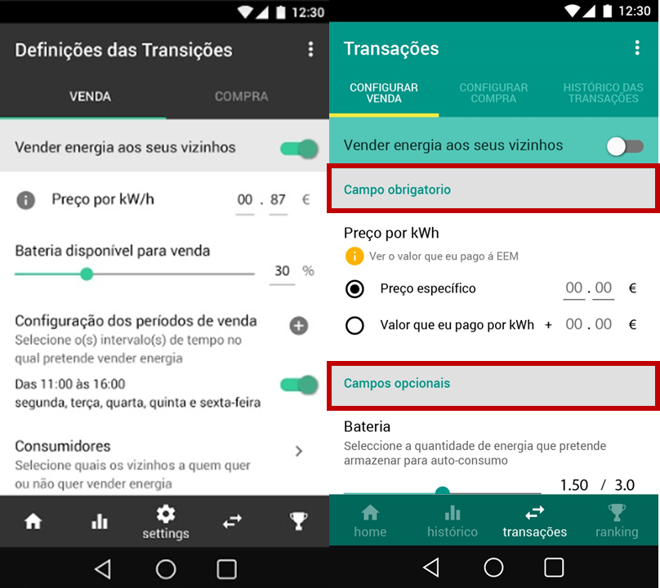
\includegraphics[width=0.7\textwidth]{./Images/ps1}
\caption{Sell settings layout before and after heuristic evaluation}
\label{fig:ps1}
\end{figure}


At the end of each user test, participants were also asked for comments and opinion about their experience. Through their feedback other two issues were identified:

\begin{itemize}
    \item Many participants said that they didn't really get why the list of transactions and transactions setting were separated, thus we decided to combine them in a single section \cref{fig:ps2}.
    \item Some participants raised possible privacy concerns about sharing with the community information about the amount of renewable energy they used. For this reason, we decided to make it possible for them to not share this information.
\end{itemize}


\begin{figure}[h]
\centering
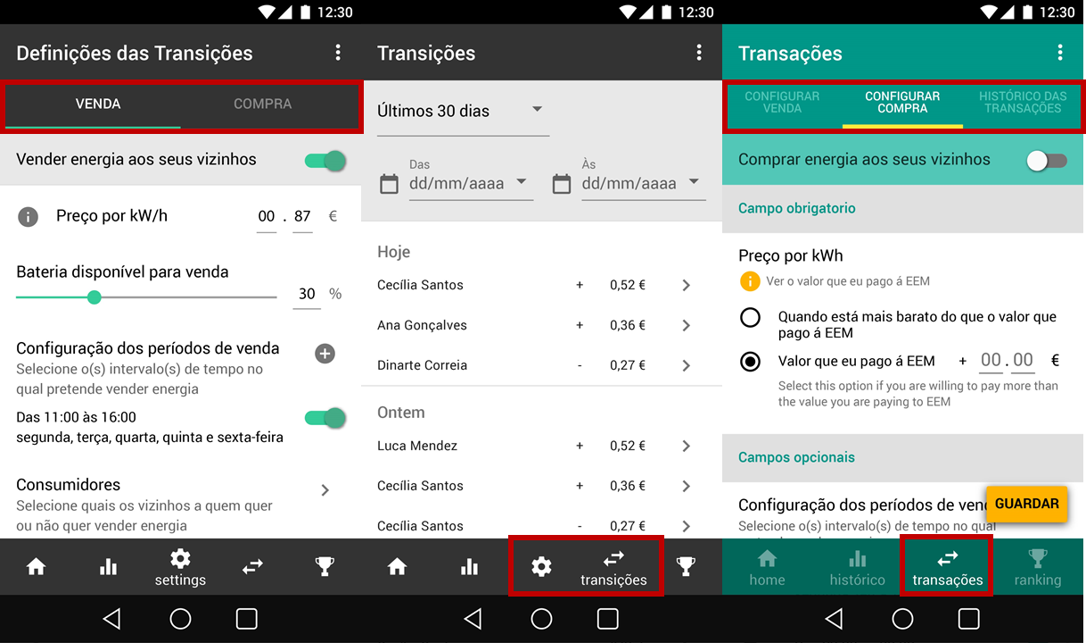
\includegraphics[width=1\textwidth]{./Images/ps2}
\caption{Sell settings/historical tradings layout before and after heuristic evaluation}
\label{fig:ps2}
\end{figure}

On the basis of the above-mentioned results, another low-fi prototype was designed and tested with different subjects. The changes made resulted resulted in the improvement of users performance allowing us to start designing the \ac{UI} mockup.

In terms of flow, we tried to keep the registration process as quick as possible. Creating a new account requires three main steps (see \cref{fig:ps3}):
\begin{enumerate}
    \item Defining users credentials: first and last name, email address and password;
    \item Input some basic information about the contract with the energy provider: voltage range, contracted power, electricity tariff and cycle (only if applicable). Here, according to the feedback from the pilot test, the information buttons showing where to find such information on the electricity bill were emphasized.
    \item Defining user typology (consumer or prosumer). In case the user registers as a prosumer, I’ll be asked to input further information concerning solar panels and battery owned.
\end{enumerate}


Before finishing the registration, users receive an IOTA seed\footnote{In a real case the user could use a seed if he already have one or generate one in the app. For this study we create the accounts and pre-charge them and only ask the user to set out a password to cipher the seed and store it.}, which gives them access to their IOTA account. Users are thus asked to set a password for that seed.
During the registration process, the user is asked to allow or not the app to share within the community the share of RES in his/her overall energy consumption. Whatever choice they make, a dialog informs them that they can always provide or deny permission anytime, by accessing their account settings. In addition, at the end of the registration, the user is provided with the opportunity to select the “automatic settings” for the buying and selling criteria. By selecting the automatic settings, users will immediately start trading energy while, if they choose the manual mode, they have to set the buying and selling criteria in "transactions" before being able to trade. Also, in this case, users are informed that they can modify this choice at any time through their account settings.

\begin{figure}[h]
\centering
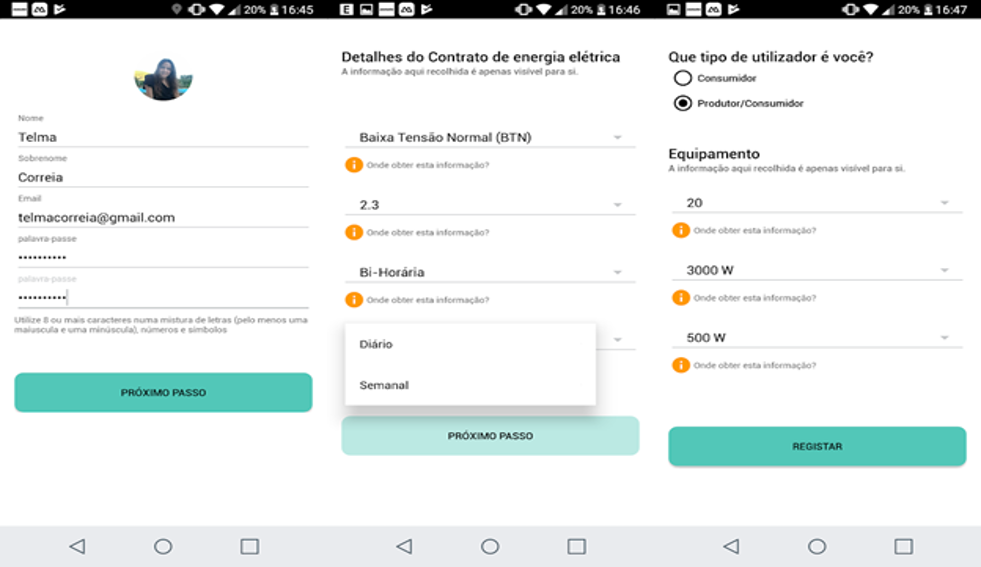
\includegraphics[width=1\textwidth]{./Images/ps3}
\caption{Registration layouts}
\label{fig:ps3}
\end{figure}


Once the user is finally registered, (s)he can access the four main feature of the app \cref{fig:ps4}.


\begin{figure}[h]
\centering
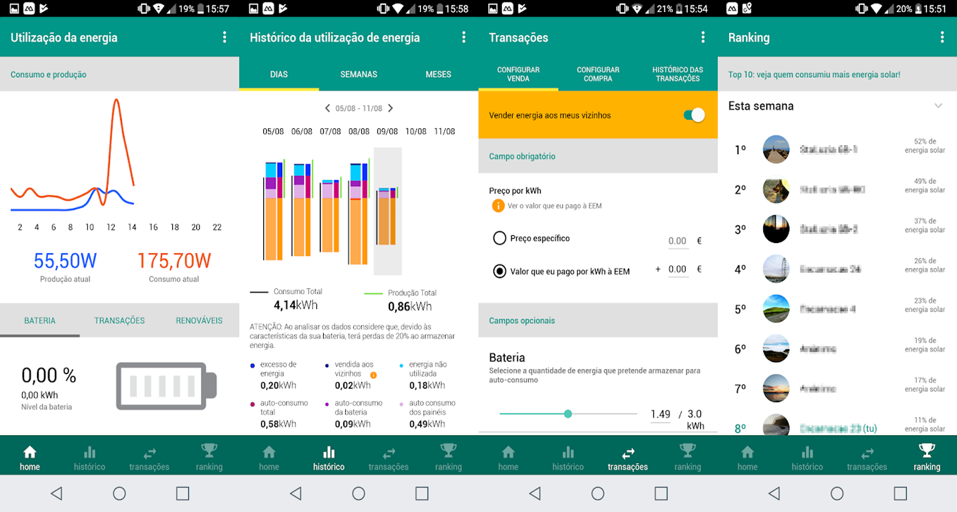
\includegraphics[width=1\textwidth]{./Images/ps4}
\caption{Main Power Share menus}
\label{fig:ps4}
\end{figure}


\textbf{Home:}
The home provides information about (\cref{fig:ps4}, 1st on the left):
\begin{itemize}
    \item current production and consumption (line chart on the top of the screen);
    \item the battery status (amount of energy stored) (\cref{fig:ps5}, 1st on the left);
    \item a summary of transactions carried out that day. Such information is presented through a heat map so to help the user identify at a glance at what time of the day (s)he buys and sell more energy. Further details about each transaction can be accessed by selecting the green arrow on the top of the heat map (\cref{fig:ps5}, the image in the middle);
    \item the share of RES in the user weekly energy consumption (\cref{fig:ps5}, 1st on the right): here the user can quickly check how much RES is using in the current week (donut chart) and how is (s)he doing in comparison to the other users (ranging from “very good”, represented by a smiling face, to “you should do better”, represented by a frowning face). The comparison with other users is always coupled with an encouraging sentence, in order to avoid a negative feedback. Data are updated every minute.
\end{itemize}

\begin{figure}[h]
\centering
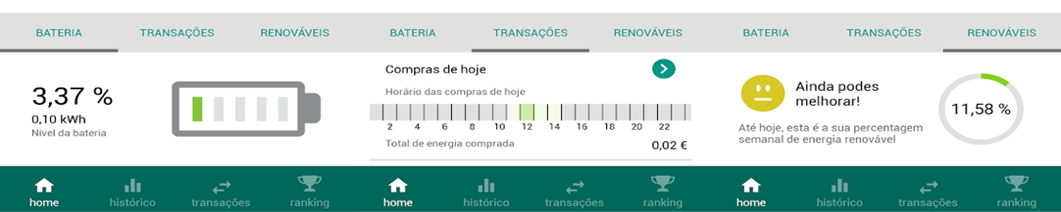
\includegraphics[width=1\textwidth]{./Images/ps5}
\caption{Home menu tabs}
\label{fig:ps5}
\end{figure}
\textbf{Histórico:} (\cref{fig:ps4}, 2nd on the left)
Through this feature, users can access their own past consumption and production data, with three levels of temporal granularity (days, weeks, months). The information is illustrated through a stacked bars graph as well as a table (on the bottom of the graph, which also serves as a legend to the graph). Not only overall production and consumption are presented, but also their respective breakdown (e.g. consumption is divided in energy bought from the supplier, from neighbours, and from self-consumption), so the user can leverage this information to modify his/her buying and selling criteria (if needed).
\Cref{fig:ps6} represents an example the information presented to users in the “histórico”.

\begin{figure}[h]
\centering
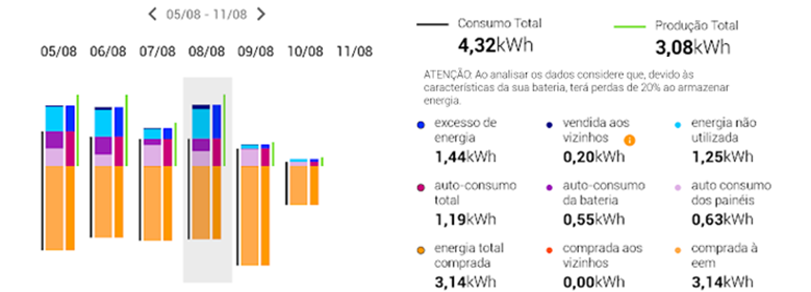
\includegraphics[width=0.7\textwidth]{./Images/ps6}
\caption{Historical daily graph}
\label{fig:ps6}
\end{figure}


As shown in \cref{fig:ps7}, for each time frame (a day, a week, or a month), the user is provided with the following information:
Energy surplus (a) and its breakdown: surplus sold to neighbours (a1) and surplus stored in the battery (a2);
Self-consumption (b), divided in direct consumption (b1) - from solar panels - and consumption from the battery (b2). This, in order to help users understanding the percentage of total battery capacity needed to fulfill their energy need and, consequently, the amount of energy they can sell to neighbours.
Energy purchased (c) and its breakdown: purchased from \ac{EEM} (c1) and from neighbours (c2).
In addition, to help users compare their total production (d1) and consumption (d2), two small line have been added to the graph.

\begin{figure}[h]
\centering
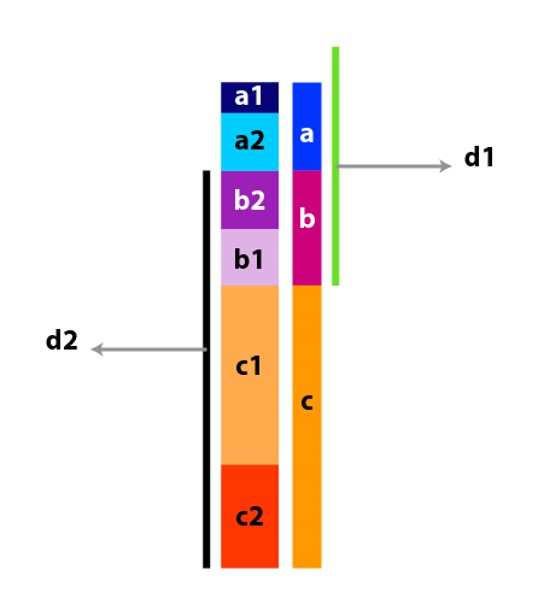
\includegraphics[width=0.5\textwidth]{./Images/ps7}
\caption{Graphical explanation for each column}
\label{fig:ps7}
\end{figure}


As shown in  \cref{fig:ps6}, the graph is always combined with a table which serves as a legend for the graph itself and provides detailed information about energy use so to prevent the user to misinterpret the visualization or, even worst, think there is something wrong with the data. For example, a user could get confused noticing that total production (green line) always exceeds the sum of “energy surplus” and “self-consumption”. An alert in the table explains that this is due to the fact that when using a Battery Energy Storage System there is always a loss of energy (about 20\%)\footnote{This is better explained in the \ref{psetms}}. In addition, in case the energy sold to neighbours and/or stored in the battery exceeds the “energy surplus” of that day/week/month, through an info button the user is provided with an explanation for that - i.e. there was still energy stored in the battery from the previous day/week/month.
Last but not least, every time the battery is full, an alert button will appear (\cref{fig:ps8}). If the user presses it, a dialog opens up and warns him that he is “wasting” his production because cannot store energy in the battery anymore.


\begin{figure}[h]
\centering
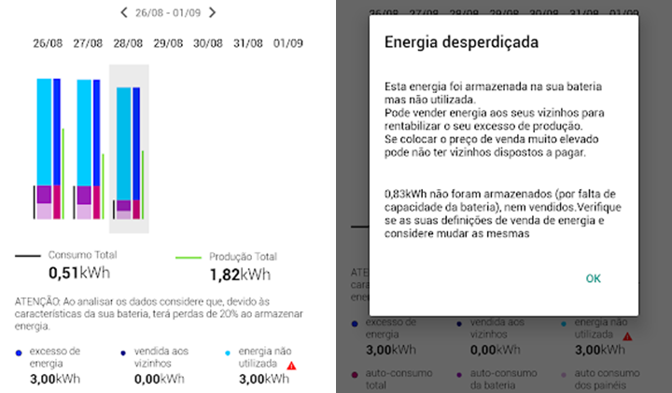
\includegraphics[width=0.7\textwidth]{./Images/ps8}
\caption{Example of wasted energy alert}
\label{fig:ps8}
\end{figure}


\textbf{ Transações: buying/selling criteria:} (\cref{fig:ps9})

This section is divided into three main sub-sections: 1) manual definition of criteria for selling energy; 2) manual definition of criteria for buying energy; 3) list of all transactions performed.
The core of the application is the manual definition of buying/selling criteria. The only mandatory field here is “price for kWh”. The user is indeed required to define at what price (s)he is willing to buy as well as sell energy. In both cases, two are the possible options: 1) a fixed price (“maximum” fixed price in the case of buying criteria); 2) a price tied to the cost of energy he/she buys from the electricity company (in the case of Madeira it is \ac{EEM}). The latter option is targeted to consumers that are subjected to dynamic pricing (i.e. have a bi-horária or tri-horária tariff), thus pay energy at different prices at different times of the day. Concerning “energy selling”, such price could be equal or bigger to the cost of energy (s)he buys from \ac{EEM} at a given moment while, regarding “energy buying”, the users set a maximum price which could be equal or lower than the cost of energy bought from \ac{EEM} at a given time. Results from the \ac{SINAIS} project revealed that many consumers are not aware of the cost of energy and, sometimes, don’t even know their own tariff. Therefore, in order to support users in defining the price for the energy they are buying and/or selling, an “information button” was added, which opens up a dialog providing information about the user’s tariff and relative energy prices. 
In both “energy buying” and “energy selling” sections there are then the following optional criteria:
\begin{itemize}
    \item Select one or more specific time frames for buying and/or selling energy;
    \item Select people you want to trade with (buy from and sell to) among the users in the community. Every time someone joins the community, all users that decided to trade only with specific people receive a notification (\cref{fig:ps10}), so they can include or not the new user among them. 
    \item Save part of the overall storing capacity of your battery for self-consumption only (this criterion is available only for energy selling). 
\end{itemize}


\begin{figure}[h]
\centering
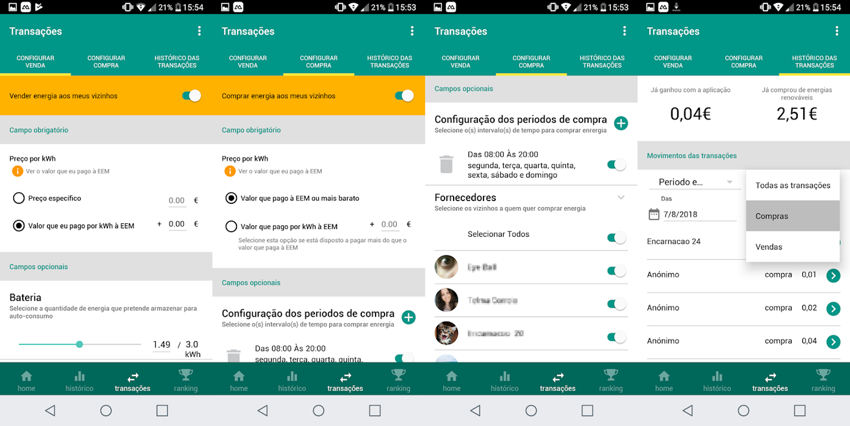
\includegraphics[width=1\textwidth]{./Images/ps9}
\caption{Power Share: Sell/Buy Settings layouts}
\label{fig:ps9}
\end{figure}

If users do not set any of the above mentioned optional criteria, (s)he will be notified that, for instance, (s)he is going to buy energy from anyone and at any time. Once all the parameters are defined, the user can start trading energy by using the slider on the top of the screen. In the same way, the user can momentarily disable the trading while keeping his/her settings as such.
The list of transaction (\cref{fig:ps9}, last one from left to right) users can quickly see their total earnings/expenses and all transactions (s)he carried out.  The list could be filtered by date range and/or by type of transaction (buying or selling). Further details about each transaction are also provided.  



\textbf{Ranking}
Here it is presented the rating for top 10 users (among those who allowed the app to display such information) with the biggest share of RES consumption. The current user place appears always in the list even if (s)he is not in the top 10.

An overflow menu is placed in the top app bar, which allows the user to access some secondary features:
\begin{itemize}
    \item Account settings;
    \item Privacy Policy;
    \item IOTA wallet.
\end{itemize}


\begin{figure}[h]
\centering
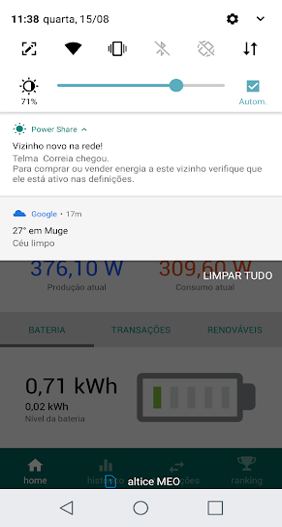
\includegraphics[width=0.3\textwidth]{./Images/ps10}
\caption{New neighbour notification}
\label{fig:ps10}
\end{figure}

\subsection{Implementation}

The rationale behind a developing a mobile application for android is that it is  more versatile and accessible since android is an open source system. In order for the app to quickly respond to changes, the Model View-ViewModel (MVVM) design pattern was adopted. This pattern has 3 main layers and lots of advantages:
\begin{itemize}
    \item \textbf{The View:} it basically consists in the layout of each screen. The View is responsible for informing the View Model Layer about the user’s actions;
    \item \textbf{The View Model} takes care of relevant data for the View layer;
    \item \textbf{The Data Model}, which is a data source abstraction. The View Model Layer works with the Data Model to get and save the data. 
\end{itemize}

A clear advantage of this pattern is the abstraction between the domain logic and presentation layer. It also makes the code easier to maintain, test and extend. \ac{MVVM} was used together with RxJava, a Java implementation of Reactive Extensions\footnote{\url{https://github.com/ReactiveX/RxJava/wiki}}, which consists in a library for composing asynchronous and event-based programs by using observable sequences.
Other relevant libraries used to develop the app are listed below:
\begin{itemize}
    \item Dagger: a fully static, compile-time dependency injection framework for Java and Android\footnote{\url{https://google.github.io/dagger/}};
    \item Retrofit\footnote{\url{http://square.github.io/retrofit/}}: a library for HTTP-client connections;
    \item MPAndroidChart\footnote{\url{https://github.com/PhilJay/MPAndroidChart}}: Chart views for Android;
    \item Firebase\footnote{\url{https://console.firebase.google.com/}}: Cloud messaging (notifications);
    \item IOTA API\footnote{\url{ https://github.com/iotaledger/iota.lib.java}}: Java wrapper around IOTA.
\end{itemize}


The \ac{UI} was designed mainly for mobile phones, nevertheless, the layout is fully responsive so it perfectly adapts to tablets. The only requirements for the application to run is a mobile device running Android 4.4.2 or higher with \ac{API} level greater or equal to 19. 


The most crucial feature implemented for the purpose of this project is the IOTA payment. As explained before, each user is provided with a seed that gives him/her access to an IOTA account. Such seed needs to be securely stored.,  Therefore, the user is required to set a password for it (\cref{fig:ps11}, first image) and only then, the seed ciphered is stored in the server. For security reasons, the deciphered seed cannot be stored on the mobile device, consequently, payments cannot be fully automated and each time a user wants to access the wallet (“ver o meu saldo”), (s)he is asked for the password set. Once the password is inputted the seed is deciphered and can be used (the seed stays only deciphered in memory, is not stored deciphered in a persistent way) .


\begin{figure}[h]
\centering
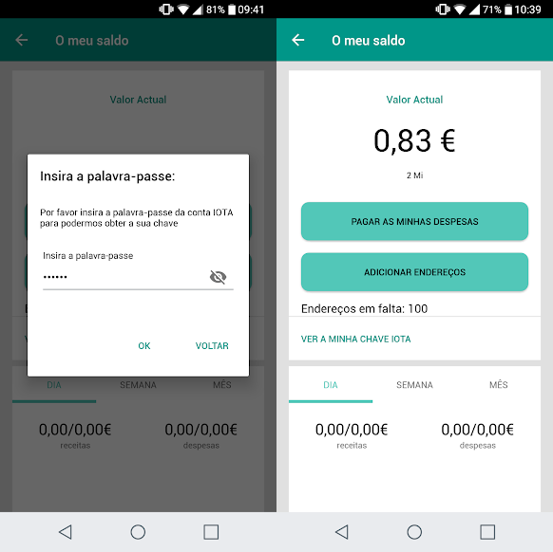
\includegraphics[width=0.3\textwidth]{./Images/ps11}
\caption{IOTA wallet in Power Share}
\label{fig:ps11}
\end{figure}

Through the wallet, users can check their account details (e.g.balance; daily, weekly and monthly incomes/outcomes).



The query for balance information could take a while to be executed, depending on IOTA node state. The same might happen when the user generates  new destination addresses (see \cref{seciotatech}). With this respect, it should be pointed out that each transaction carried out by the user as seller requires a new address. When (s)he runs out of addresses, receives a push notification and an email asking to generate new addresses. To make the payment, the user has to press the “pagar as minhas despesas” button. If the user has not enough balance, the payment will be rejected by the node. It is, of course,  user responsibility to have enough balance to keep trading.


Since the application has no database, SharedPreferences is used to persistent store user tokens (Bearer token and Firebase token), therefore it does not work in offline mode. 


% #############################################################################
\section{Power Share Energy Trading Management System}\label{psetms}


\Cref{fig:ps12} shows an overview of the ETMS (the integration of IOTA technology in the ETMS will be explained in the next section). The Android application is connected with the ETMS, which in its turn is connected with the smart meters providing information about energy production and consumption for each user. Both communications are made by a REST API using the https protocol with authentication. The https protocol was used for security reasons, like prevent man--in--the--middle attacks -- i.e. an attacker alters the content of the messages sent between the application--server and smart meters-server.
The ETMS was built using java with Spring framework, this option was considered regarding their advantages like the embedded Tomcat (java web server), following the \ac{MVC} architecture given the maintainability, testability, and scalability of this approach. The database used is MySql.


\begin{figure}[h]
\centering
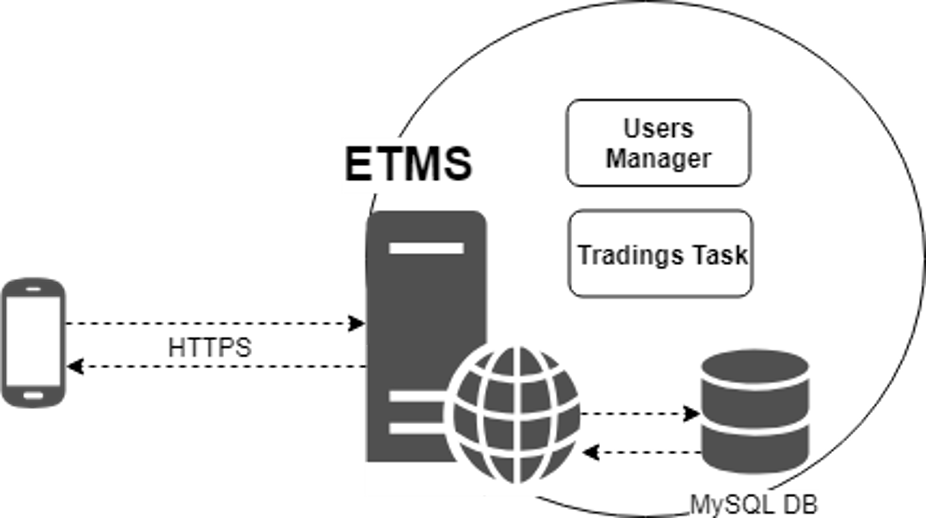
\includegraphics[width=0.9\textwidth]{./Images/ps12}
\caption{Power Share \ac{ETMS} architecture}
\label{fig:ps12}
\end{figure}

%%%%%%%%%%%%%%%% REFER ATTACHMENTS %%%%%%%%%%%%%%%
The Users Manager layer contains all the endpoints (\cref{chapter:appendixA}) available for an authenticated client. The authentication scheme used is Bearer Authentication, that is part of OAUTH 2.0\footnote{Authorization protocol that gives an \ac{API} client limited access to user data on a web server.} in RFC 6750\footnote{\url{https://tools.ietf.org/html/rfc6750}}. This Bearer token is generated on the login request and has to be used by the client in the “Authorization header” for all endpoints (except login and register). The \ac{API} requests used to feed the client application are GET, POST, UPDATE and DELETE. The full \ac{UML} database schema, with all parameters of each table and respective relations, can be found in \cref{chapter:appendixB}. From now on, any reference to a database table can be founded in that schema. 


A trading is the combination of three main asynchronous tasks. “Start transactions” (\cref{fig:ps13}), “Verify transactions” and “Stop Transactions” (\cref{fig:ps15}).

\textbf{Start Transactions:} Once a user has set his parameters for trading energy and activated the trading by sliding the switch to the on position, an entry with user id and sales/bough settings id are added in the database (in want\_sell or want\_buy table respectively). Such a combination of user id/settings id is unique. When the user starts a transaction or turns off the trading switch, this entry is removed from the table. Each minute the system verifies if there are entries in the want\_sell table and, for each entry found, the server runs the match algorithm to find a buyer whose demand for energy matches the seller settings - e.g. a seller that offers solar energy to neighbours at the same price (s)he pays energy to \ac{EEM} (let’s imagine, (s)he has “simples” tariff thus pays always 0,1629 € per kWh) will match and thus being able to trade with a consumer who has selected a maximum buying price that is equal or higher than 0,1629€/kWh. 

\begin{figure}[h]
\centering
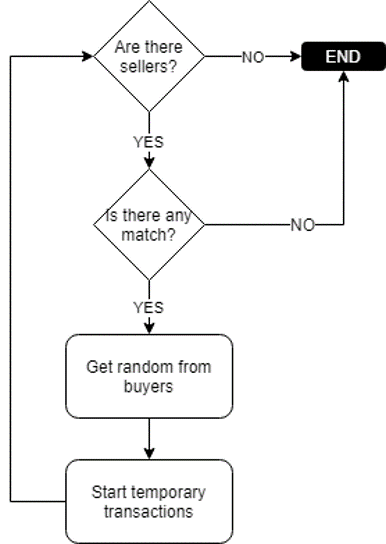
\includegraphics[width=0.4\textwidth]{./Images/ps13}
\caption{Start Transactions flow chart}
\label{fig:ps13}
\end{figure}

So, by selecting a specific selling price, sellers are guaranteed they will always sell energy for neither more nor less than that price. On the contrary, buyers cannot know in advance the actual amount they will pay for kWh. They are only guaranteed it will never be higher than the one they have set. In order to ensure impartiality, both sellers and matching buyers lists are shuffled. Every time the system finds a match, a temporary transaction is created, while the fields corresponding to the amount of energy consumed (by the buyer)  and remaining surplus (of the seller) are updated in the database. The transaction duration is configurable, however, we set one hour as a fixed time to perform each transaction. This choice was made after the analysis of historical consumption and production data of our users which lead us to conclude that, in less than one hour, the amount of energy exchanged could easily be so low  that the rounded value presented to the users is likely to be zero. 





\textbf{Verify transactions:} A possible scenario is that a seller has the trading on but no energy stored in the battery to sell. For this reason, every two minutes the system runs a verification transactions task (\cref{fig:ps14}). By performing this task, it verifies if the consumed energy in a temporary transaction is greater than zero (the system only verifies transactions running over five minutes). In case the value of a transaction is not higher than zero, it will be immediately stopped. The respective entry in the temporary\_transactions table is deleted and want\_buy and want\_sell tables are again updated.


\begin{figure}[h]
\centering
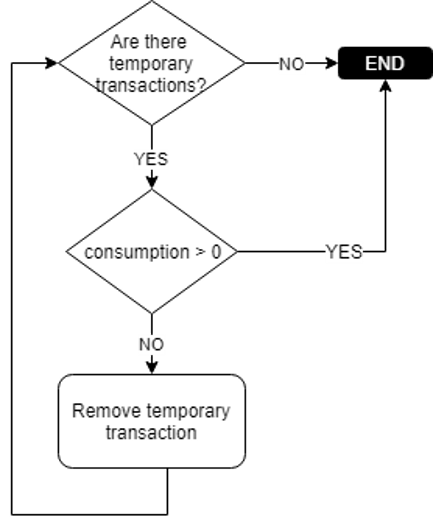
\includegraphics[width=0.4\textwidth]{./Images/ps14}
\caption{Verify Transactions flow chart}
\label{fig:ps14}
\end{figure}


\textbf{Stop Transactions:} This task consists in stopping all transactions with the duration equal to one hour. When a transaction ends, the system verifies if the energy actually used  by the buyer corresponds to the requested amount. In other words, the system verifies if the surplus energy made available by the seller is enough to meet the demand from the buyer and, in case it is not, updates the actual amount of energy traded accordingly. This can be done only at the end of the transaction due to concurrency restrictions, i.e. it is not guaranteed to have data from the buyer and the seller’s meters at the same time. The system is designed to not  stop any transaction if data is missing. In case the connection between the server and the smart meter should fail, the transaction won’t be stopped, i.e. none transactions is stopped if the last timestamp received by the buyer and/or seller’s meter is earlier than the end of the transaction (\cref{fig:ps15}). This is possible because the smart meter sends the data points sequentially.



\begin{figure}[h]
\centering
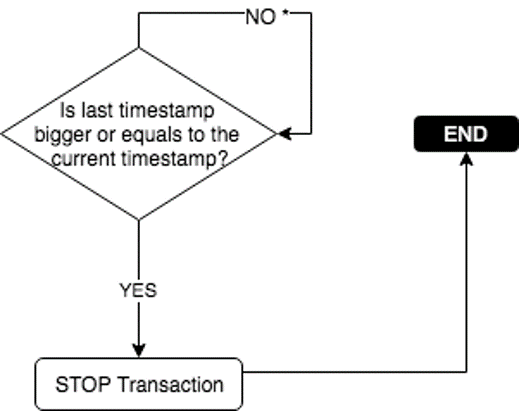
\includegraphics[width=0.4\textwidth]{./Images/ps15}
\caption{Stop Transactions flow chart}
\label{fig:ps15}
\end{figure}


At the end of each transaction, the system verifies if the seller has any available address for it and, if so, it associates the address with that transaction (\cref{fig:ps16}). If no address is available an asynchronous routine named \textbf{Transactions Addresses} task will be performed. This routine runs one time a day. It basically verifies if there are sales without an associated address and, in case it finds some, it will notify the respective users (sellers only) the need to generate new addresses for getting paid. This alert consists in an email and a push notification received directly on the mobile device where the app is installed.  



\begin{figure}[h]
\centering
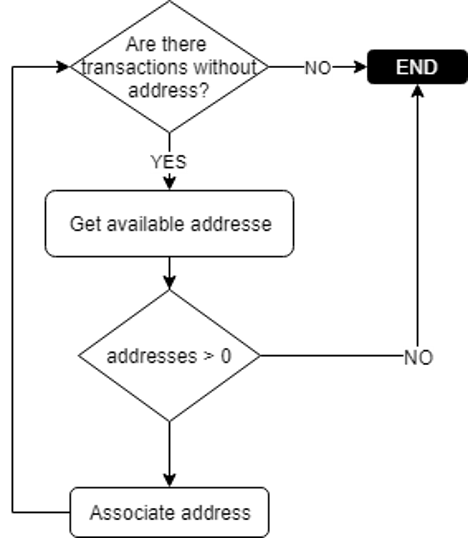
\includegraphics[width=0.4\textwidth]{./Images/ps16}
\caption{Transactions Addresses flow chart}
\label{fig:ps16}
\end{figure}

\subsection{Battery Simulation}

Technically, to trade energy by using this system, a prosumer does not need to have a \ac{BESS} (i.e. in the moment there is excess production and if there is demand, the the energy surplus can be sold in real time). However, having a \ac{BESS} will exponentially increase the effectiveness of this system, since users can store the energy surplus throughout the day and sell or use it later. For this reason, and since none of the participants in the field test have a battery, for the purpose of this study the system will simulate a 3000w “virtual battery” for each of them. Before explaining how this simulation is done, the following  information about a Battery Energy Storage System need to be provided:
\begin{itemize}
    \item The battery capacity represents the amount of energy that it can store (in kWh). Capacity is different from the power rating, which on the contrary represents the amount of energy (kW) a battery can provide in a given time frame.
    \item The \ac{DOD} defines the degree to which a battery is discharged in relation to its total capacity . In order to not compromise the battery lifetime, it should never reach 100\% or 0\% (the optimal \ac{DOD} should range between 20\% and 80\%). For the purpose of our study, in order to simplify the server logic we did not set a maximum and minimum \ac{DOD} for our “virtual batteries”;
    \item Batteries consume energy too. The \ac{RTE} is the term used to describe how much of the energy stored in the battery is lost in a “round trip” between the time the energy storage system is charged and then discharged \cite{energymag}. The \ac{RTE} of our virtual batteries is 80\% (i.e. 20\% of the energy stored is lost).
\end{itemize}

In this respect, in order to faithfully simulate the behaviour of an actual battery, the system  multiplies the amount of energy stored in the virtual battery by its \ac{RTE} (i.e. energy stored x 0,8), so to get the amount of energy available for trading. No losses are calculated on the amount of energy sold.
% #############################################################################
\section{IOTA integration} \label{ii}
Blockchain technology, more precisely IOTA, is used here as a payment system. For this purpose, \ac{IRI} was run on a Ubuntu 16.04.4 server equipped with a 6 cores processor and 8GB RAM.



Each node on the Tangle runs \ac{IRI} and needs other neighbours (i.e. other nodes running \ac{IRI}, which can be found on the official IOTA discord channel\footnote{\url{https://discordapp.com/invite/rYA7gFa}}) to perform a transaction.  Our node has three neighbors. In other words, the Tangle works as follow: one node performs a transaction and pays for it by validating two other non-validated transactions, called Tips, following the “Tip Selection” process. In order to validate the Tips \ac{IRI} issues the Tip Selection Algorithm Deep Dive that “has to walk a portion of the Tangle (subgraph) twice, stepping according to a rating calculation, selecting an entry point for each walk.”\cite{iotatips}. Since a user has to validate two transactions to get his one approved an efficient network is required, therefore the more active users in the network the better. In addition, it must be pointed out that, in order to perform the tips validation properly, neighbors need to be synchronized with the Tangle, run over a good machine (i.e. a powerful computer that, according with IOTA recommendations, should be at least equipped with a 2 cores processor and 4GB RAM) and have a stable network of neighbors in their turn. For this reason, we only know if a node is good or not by adding it as a neighbour and testing the network behavior. 


This way we can perform transactions using the Tangle through the IOTA \ac{API}, having a decentralized network operated by the Tangle that validates transactions between neighbors. Despite there are many public nodes available, we decide to run our own node since, if a public node becomes unstable, we don't have the possibility to fix it and consequently cannot guarantee the transaction will be performed successfully.  \ac{PS} relies on this node to perform the payments and the \ac{POW} is done as a service by the application. The POW on the Tangles is simpler compared to, for instance, the Bitcoin \ac{POW}, therefore it requires less computational power.



The energy traded is paid through IOTA cryptocurrency (MIOTA). For the purpose of our study, a given amount of MIOTA (around 10€) has been pre-purchased for each participant. It is then their responsibility to verify that the balance in their iota account is enough to keep trading. If the user runs out of MIOTA, the system will automatically disable the trading. 


As explained before, in order to get paid for the energy sold, the user needs to generate an address and it is his/her responsibility to do so. On the Tangle, one address could receive funds more than once, however, since we sent a transaction with specific address as input, we should never use that address again. Indeed, IOTA uses winternitz one-time signatures, which degrade security exponentially after each use of the same address \cite{iotaseeds}.




% If Printing on DOUBLE SIDED pages, the second page should be white.
% Otherwise, comment the following command:
\cleardoublepage
%
%Chapter 4
% #############################################################################
% This is Chapter 4
% !TEX root = ../main.tex
% #############################################################################
% Change the Name of the Chapter i the following line
\fancychapter{Evaluation}
\cleardoublepage
% The following line allows to ref this chapter
\label{chap:evaluation}
This chapter describes the methodology adopted to test the Power Share mobile application with real users. Data resulting from the users’ test are presented. 

\section{Methodology}

The evaluation of Power Share app has three main goals:


\begin{enumerate}
    \item Assessing the usability of the system;
    \item Assessing users acceptance of energy trading in Madeira Island to understand if it could be a viable future business model for the SMILE project;
    \item Evaluating users understanding and attitudes toward adoption of blockchain as a payment method.
\end{enumerate}


The methodology selected for assessing the aspects mentioned above includes semi-structured interviews (to be performed after the one-month test) and monitoring users’ interactions through the Fabric.io platform. Due to time constraints, the start of the field test has been postponed thus, results from the semi-structured interviews cannot be included in the present document (but will be presented during the viva). 


\subsection{Semi-structured interviews}

The interviews with the participants in the field test are scheduled to start mid-October. Each interview should last around one hour and will be performed with the support of researchers from the Madeira-Interactive Technologies Institute.
The main topics to be covered during the interviews are:
\begin{itemize}
    \item Understanding and perception of the system (e.g. perceived usefulness);
    \item Actual use (i.e. how they used the app);
    \item Behavioral intention (i.e. their willingness to use the app/system in the future);
    \item Usability (e.g. perceived ease to use);
    \item Their perception of using blockchain as a payment method.
\end{itemize}

\subsection{Monitoring users’ interactions}

To further understand how participants used the application, their interactions have been monitored using Fabric.io. 


Specifically, data collected concern:
\begin{enumerate}
    \item \textbf{Daily usage of the application:} number of daily interactions, which features they accessed and at what time;
    \item \textbf{Performance of the app:} i.e. crashes;
    \item \textbf{Trading settings:} if and how users set criteria for buying and selling energy;
\end{enumerate}

\subsection{Procedure}

To assess the system, we decided to run a small pilot in Madeira island, asking prosumers to use the application for a month. Initially, ten households in Funchal were recruited, but at the end, only nine of them participated in the field test (one decided to withdraw his participation).
 Before performing the study, informed consent was provided to participants. Then the research team, supported by local technicians, verified the existing communication infrastructure (internet connection) and installed the required equipment to collect production and consumption data (smart meters). Also, an Android tablet was provided to those participants that did not have a mobile device able to run the app.

At the end of August, an email with instructions to download and install the app was sent to all participants. The application was launched on September 1st. Not all users installed the app immediately, thus a reminder email was sent to those users who still had to create an account.
 Every weekend, each user received via email a summary of his weekly production and consumption breakdown (an example of the weekly summary can be founded in the \cref{chapter:appendixC}).
 
 \section{Results}
 As expected, data collected through Fabric.io (\cref{fig:gr1}) show that the most used feature was the home (real-time feedback). According with literature on \ac{EF}, real-time feedback is the information users are more interested in, thus the application was designed to show this screen by default every time a user launches the app. For this reason, the high score of real-time feedback (which was used over 100\% times more than the second most used feature) is not enough to confirm users interest for it and thus needs to be addressed during the interviews. Interestingly, the second most popular feature was the ranking. This result supports findings from previous studies on \ac{EF}, which demonstrate the effectiveness of social comparison. “Ranking” is followed by  “Histórico” (self-comparison). On this respect, it should be pointed out that daily and weekly data received more or less the same attention from users, while monthly data was not very popular (likely because the study lasted only one month).


Despite most of the users selected the “automatic settings” for trading energy,  they did access trading settings and a list of transactions several times. This result suggests a certain degree of curiosity from users about energy trading, which definitely has to be further investigated during the interviews. Another interesting result is the lack of interest in the “IOTA wallet”, which was the less popular feature together with “account settings”. This could be due to the fact that both “IOTA wallet” and “account settings” were hidden compared to the other features of the app since accessible only from the overflow menu placed in the top app bar. Nevertheless, this result needs to be further investigated during the interviews since it could represent a lack of interest or understanding of payment via blockchain. 

 
 \begin{figure}[h]
\centering
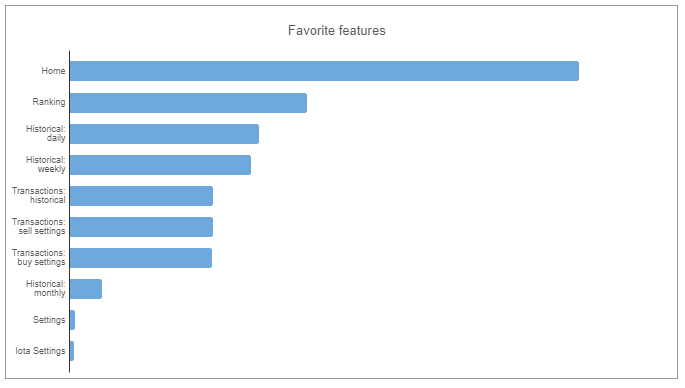
\includegraphics[width=0.8\textwidth]{./Images/graph1}
\caption{Favorite features based in the number of accesses}
\label{fig:gr1}
\end{figure}

Users motivations behind results reported above will be investigated during the interviews. Especially, what needs to be clarified is the reason that led the majority of users to select the “automatic settings” for trading energy, since it could be due to a usability issue (during the pilot test, the manual setting task was defined as the most demanding).  

\Cref{fig:gr2} shows the number of accesses to the app throughout the study. No significant correlation has been found between number of accesses and day of the week (included weekend vs. weekdays). Also, surprisingly, push notifications and weekly summary did not affect the use of the app.. 


 \begin{figure}[h]
\centering
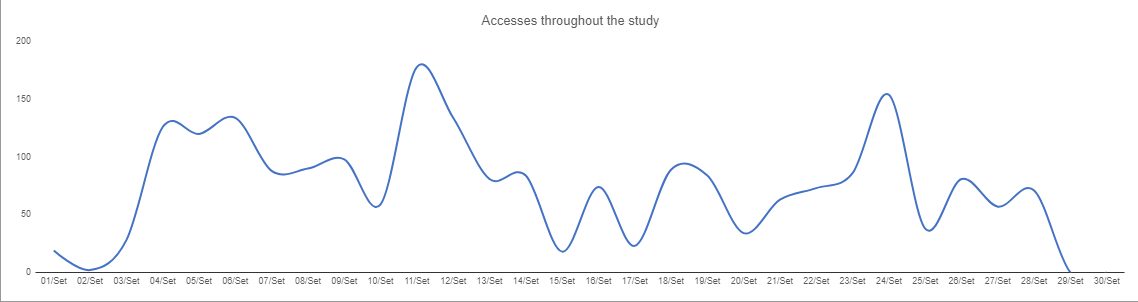
\includegraphics[width=0.8\textwidth]{./Images/graph2}
\caption{Application accesses throughout the study }
\label{fig:gr2}
\end{figure}

Each user’s session lasted an average of 2 minutes and 15 seconds. In agreement with the literature on EF, interaction with the system decreased over time (\cref{fig:gr3}). 


 \begin{figure}[h]
\centering
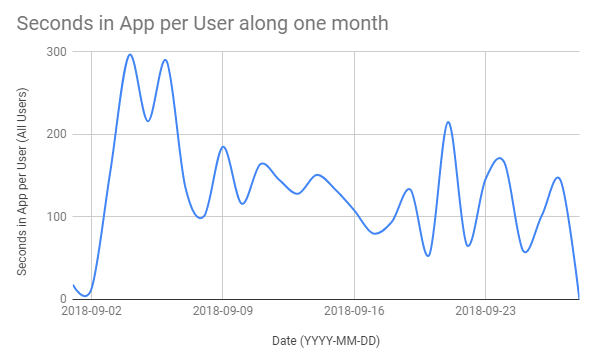
\includegraphics[width=0.8\textwidth]{./Images/graph3}
\caption{Seconds in the Application throughout the study}
\label{fig:gr3}
\end{figure}

Regarding the energy trading (\cref{tab:tr}), we recorded a daily average of 19 transactions, which means more than 2 transactions a day per user. 
At the end of the study, a total of 349 transactions were performed, the corresponding to about 45.1 kWh of energy shared between the users. 



The main bottlenecks identified regard the payment system. As already explained in 3.2.2, to pay for the energy received, users have to press the “pagar as minhas despesas” button in their “IOTA wallet”. In the server, a transaction could have three different states: “not-attached” (not paid), “attached” (after the user presses the pay button), and “validated” (when the payment is performed successfully). At the end of the study, all transactions were “not-attached”, which means that none of the users have understood they were required to allow the payment manually. The choice of recording the “attached” state is due to the fact that the payment through IOTA is very slow, which could therefore lead the user to close the application before the process is completed (thus leading to interrupt the payment). By recording this intermediate state, we have been able to verify if users tried to make payments. In addition, none of the users have generated the destination addresses, which are required to receive a payment. These two bottlenecks suggest the need to redesign the payment process by increasing the level of automation and/or adding affordances to help users performing the required actions.

\begin{table}[htb]
\centering
\normalsize
    \caption{Transactions data during the study}
    \label{tab:tr}
{\footnotesize
    \begin{tabular}{ | c | c | c | c | }
    \hline 
    	& \textbf{Nr Transactions} & \textbf{Ammount (\euro)} & \textbf{Ammount (kWh)}\\ \hline \hline
    Average  & 19.4  &  0.41  &   2.51 \\ \hline
    Max  & 34   &  0.81  &   4.96 \\ \hline 
    Min  & 9   &  0.15  &   0.93 \\ \hline
    Total  & 349  &  7.35  & 45.12 \\ \hline
    \end{tabular}
    }
\end{table}

Throughout the study, only one crash occurred, which affected three users (\cref{fig:crash}). This crash was due to the fact that those users have run a query at midnight; in other words, they were asking the server for data with wrong intervals, thus the server returned an error and the application crashed.

 \begin{figure}[h]
\centering
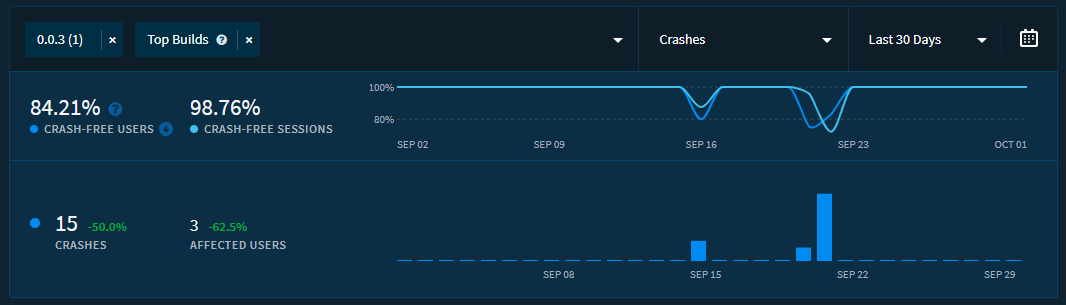
\includegraphics[width=0.8\textwidth]{./Images/crash}
\caption{Application crashes during the deployment}
\label{fig:crash}
\end{figure}
% If Printing on DOUBLE SIDED pages, the second page should be white.
% Otherwise, comment the following command:
\cleardoublepage
%
%Chapter 5
% #############################################################################
% This is Chapter 5
% !TEX root = ../main.tex
% #############################################################################
% Change the Name of the Chapter i the following line
\fancychapter{Conclusions}
\cleardoublepage
% The following line allows to ref this chapter
\label{chap:conclusions}

	
Power Share is a complete application, ready to be used. It combines a system for energy trading, that uses blockchain technology as a payment method, with a low-cost Eco-Feedback system. The application was designed building on results from the literature review, as well as on the analysis of the most relevant projects on both \ac{EFS} and \ac{ET}.
As an \ac{EFS}, Power Share provides both real-time and historical data (“Home” and “Historico”) \cite{Giulio2009}, and leverages social comparison (“Ranking”) \cite{Froehlich2010} to foster behavior change, by challenging users to increase consumption from renewables and compete against their neighbors. As demonstrated by data collected through Fabric.io, both functionalities have been highly appreciated by participants in the field test, confirming results from previous studies.
As an energy trading platform, Power Share automatically matches demand and offer, and perform the payment through IOTA. The use of IOTA is probably the main contribution of the present work. Designed for the Internet of Things, IOTA is a novel technology and Power Share, to the best of our knowledge, is the first project testing such technology for the \ac{P2P} energy market. Indeed, despite there are already several players in the \ac{P2P} energy trading market (see \cref{rps}), none of them is currently using IOTA system. The big advantage of using IOTA for payment is that it simultaneously solves scalability issues (which characterize several other blockchain technologies) and eliminates transaction fees. The last aspect, in particular, is probably the most important for those who want to develop a \ac{P2P} energy system, since transactions usually involve micropayments. In addition, IOTA has shallow resource requirements compared to other blockchains. 



Power Share differs from most of the existing projects due to the high degree of freedom it gives to users. While much \ac{P2P} energy trading applications are designed to be as much automated as possible, Power Share gives users the chance to set their criteria for trading energy and provides them with all information needed to make an aware choice (via a detailed feedback about consumption and production). Despite the majority of participants in the field test selected the “automatic setting”, adding the “manual” option allowed us to further test users’ attitude to the system and energy trading in general.
As stated before, the process of matching demand and offer is fully automated. This way, users don’t have, for example, to select the supplier that matches their buying criteria anytime they are in need of energy. Also, transactions are managed by a fair algorithm, which guarantees that all member of the community will equally benefit from the system. 



Like most of the existing projects and startups providing platforms for energy trading, also this project needs to leverage on the traditional energy grid, thus it does not include the development of a physical infrastructure for energy sharing. On this respect, it should be pointed out that the context chosen to test the system presents a great constraint which, currently, prevents the use of Power Share. As already mentioned, indeed, to protect the grid from Frequency and Voltage fluctuations, prosumers in Madeira island are not allowed to inject their surplus energy in the grid. For this reason, the energy trading has been simulated. Nevertheless, this limitation also represents the significant potential of a system like Power Share for Madeira Island. Considering a scenario where more prosumers are equipped with \ac{BESS} - a solution that is being developed and tested for the scope of SMILE project - an energy trading system, combined with specialized Battery Management Systems, could be used as a resource for balancing the grid. For example, a prosumer can sell part of the energy available in his battery to the \ac{DSO}, which can then use it to respond to a sudden increase in the energy demand.


Due to the limited duration of the field test (one month), it is not possible to test the long-term effectiveness of such a system. This is something that needs to be investigated to better understand the potential of \ac{P2P} energy trading. Unfortunately, at the time of this writing, only for one of the existing projects (Brooklyn Microgrid), it is possible to find some prior results about users acceptance of the system. Concerning the other pilot projects and startups, no information is available on this aspect, suggesting the need for further research on the impact of \ac{P2P} energy trading from a user point of view. In this respect, another limitation of this work is the lack of time for completing the evaluation with the users. The field test in Madeira was also meant to pave the way for the study of users attitude towards \ac{P2P} energy trading, which is an important aspect that still needs to be investigated. Data collected so far shows that the application has been used to perform energy trading. The fact that all users, also those that selected the “automatic setting” (and consequently, those that could have just “installed and forgotten it”), kept interacting with the app for all duration of the test is already a great result. Nevertheless, given the importance of collecting a feedback from users, the complete evaluation of the system will still be performed after the delivery of this document.
The semi-structured interviews will focus on people understanding and acceptance of blockchain technology, as well as on their perception of such technology for \ac{P2P} energy trading. From a purely technical point of view, integrating blockchain in a system like Power Share is a significant advantage, since it provides a decentralized payment method without a single point of failure, and it is reliable by itself, thus no third parties are needed. As a developer, the author feels the need to point out a weakness of the IOTA technology, that is to say, its immaturity.  Between the beginning and the end of this study until the end the IOTA technology has been upgraded, and better documentation and support material for developers released. However, due to its immaturity, several issues have arisen while testing the system. Among them, we should mention the unexpected length (concerning time) of the payment process via IOTA, which occasionally has led to the need for “re-attaching” the transaction to effectively complete the payment. This, from a developer perspective, makes the payment system difficult to implement, while for users could be quite annoying. 


\section{Future work} 


Power Share draws on novel technology and therefore there is room for improvements in several aspects. A most significant improvement that could be made regards the matching algorithm described in \cref{psetms}. The matching between the buyer and seller could be made more smartly, by considering the historical consumption and production of each user. This should be done by using machine learning algorithms. Another possible upgrade to the system consists in combining blockchain with \ac{IoT}, i.e. running the smart contract directly on connected smart devices (smart meters). This would further decentralize the process by removing the communication layer between \ac{ETMS} and the sensors.
Last but not least, the possibility to register multiple accounts for the same household, with different roles (only one admin but multiple users), as well as having multiple households under the same account, would be a nice to have featured in the future. Currently, the application allows each user to register only one account per household. Nevertheless, in a real-life scenario, all members of the household should be able, for instance, to access production and consumption data. At the same time, who also owns a summer house equipped with solar panels and a \ac{BESS}, for example, should be able to manage that installation too without the need of registering a second account. 




% If Printing on DOUBLE SIDED pages, the second page should be white.
% Otherwise, comment the following command:
\cleardoublepage
%
%Chapter 6
%% #############################################################################
% This is Chapter 6
% !TEX root = ../main.tex
% #############################################################################
% Change the Name of the Chapter i the following line
\fancychapter{Conclusions}
\cleardoublepage
% The following line allows to ref this chapter
\label{chap:conclusion}

\todo[color=green!40, author=Rui Cruz, fancyline]{You should always start a Chapter with an introductory text}{} Pellentesque vel dui sed orci faucibus iaculis. Suspendisse dictum magna id purus tincidunt rutrum. Nulla congue. Vivamus sit amet lorem posuere dui vulputate ornare. Phasellus mattis sollicitudin ligula. Duis dignissim felis et urna. Integer adipiscing congue metus.
% #############################################################################
\section{Conclusions}
Lorem ipsum dolor sit amet, consectetuer adipiscing elit. Morbi commodo, ipsum sed pharetra gravida, orci magna rhoncus neque, id pulvinar odio lorem non turpis. Nullam sit amet enim. Suspendisse id velit vitae ligula volutpat condimentum. Aliquam erat volutpat. Sed quis velit. Nulla facilisi. Nulla libero. Vivamus pharetra posuere sapien. Nam consectetuer. Sed aliquam, nunc eget euismod ullamcorper, lectus nunc ullamcorper orci, fermentum bibendum enim nibh eget ipsum. Donec porttitor ligula eu dolor. Maecenas vitae nulla consequat libero cursus venenatis. Nam magna enim, accumsan eu, blandit sed, blandit a, eros.

Quisque facilisis erat a dui. Nam malesuada ornare dolor. Cras gravida, diam sit amet rhoncus ornare, erat elit consectetuer erat, id egestas pede nibh eget odio. Proin tincidunt, velit vel porta elementum, magna diam molestie sapien, non aliquet massa pede eu diam. Aliquam iaculis. Fusce et ipsum et nulla tristique facilisis. Donec eget sem sit amet ligula viverra gravida. Etiam vehicula urna vel turpis. Suspendisse sagittis ante a urna. Morbi a est quis orci consequat rutrum. Nullam egestas feugiat felis. Integer adipiscing semper ligula. Nunc molestie, nisl sit amet cursus convallis, sapien lectus pretium metus, vitae pretium enim wisi id lectus. Donec vestibulum. Etiam vel nibh. Nulla facilisi. Mauris pharetra. Donec augue. Fusce ultrices, neque id dignissim ultrices, tellus mauris dictum elit, vel lacinia enim metus eu nunc.

Proin at eros non eros adipiscing mollis. Donec semper turpis sed diam. Sed consequat ligula nec tortor. Integer eget sem. Ut vitae enim eu est vehicula gravida. Morbi ipsum ipsum, porta nec, tempor id, auctor vitae, purus. Pellentesque neque. Nulla luctus erat vitae libero. Integer nec enim. Phasellus aliquam enim et tortor. Quisque aliquet, quam elementum condimentum feugiat, tellus odio consectetuer wisi, vel nonummy sem neque in elit. Curabitur eleifend wisi iaculis ipsum. Pellentesque habitant morbi tristique senectus et netus et malesuada fames ac turpis egestas. In non velit non ligula laoreet ultrices. Praesent ultricies facilisis nisl. Vivamus luctus elit sit amet mi. Phasellus pellentesque, erat eget elementum volutpat, dolor nisl porta neque, vitae sodales ipsum nibh in ligula. Maecenas mattis pulvinar diam. Curabitur sed leo.

Nulla facilisi. In vel sem. Morbi id urna in diam dignissim feugiat. Proin molestie tortor eu velit. Aliquam erat volutpat. Nullam ultrices, diam tempus vulputate egestas, eros pede varius leo, sed imperdiet lectus est ornare odio. Lorem ipsum dolor sit amet, consectetuer adipiscing elit. Proin consectetuer velit in dui. Phasellus wisi purus, interdum vitae, rutrum accumsan, viverra in, velit. Sed enim risus, congue non, tristique in, commodo eu, metus. Aenean tortor mi, imperdiet id, gravida eu, posuere eu, felis. Mauris sollicitudin, turpis in hendrerit sodales, lectus ipsum pellentesque ligula, sit amet scelerisque urna nibh ut arcu. Aliquam in lacus. Vestibulum ante ipsum primis in faucibus orci luctus et ultrices posuere cubilia Curae; Nulla placerat aliquam wisi. Mauris viverra odio. Quisque fermentum pulvinar odio. Proin posuere est vitae ligula. Etiam euismod. Cras a eros.

Nunc auctor bibendum eros. Maecenas porta accumsan mauris. Etiam enim enim, elementum sed, bibendum quis, rhoncus non, metus. Fusce neque dolor, adipiscing sed, consectetuer et, lacinia sit amet, quam.
% #############################################################################
\section{System Limitations and Future Work}
Aliquam aliquet, est a ullamcorper condimentum, tellus nulla fringilla elit, a iaculis nulla turpis sed wisi. Fusce volutpat. Etiam sodales ante id nunc. Proin ornare dignissim lacus. Nunc porttitor nunc a sem. Sed sollicitudin velit eu magna. Aliquam erat volutpat. Vivamus ornare est non wisi. Proin vel quam. Vivamus egestas. Nunc tempor diam vehicula mauris. Nullam sapien eros, facilisis vel, eleifend non, auctor dapibus, pede.
% If Printing on DOUBLE SIDED pages, the second page should be white.
% Otherwise, comment the following command:
%\cleardoublepage
%
% -----------------------------------------------------------------------------
% BIBLIOGRAPHY
% Add the Bibliography to the PDF table of contents (not the document table of contents)
\pdfbookmark[0]{Bibliography}{bib}
% The bibliography style sheet
% Chose your preferences on the format of the entries and the Labels:
% IEEEtran: Used in general (recommended for IST Thesis)
%           Entries are labelled and sorted by appearance in the document
%           Labels are Numeric inside square brackets
\bibliographystyle{IEEEtran}
%
% Apalike:  Entries formatted alphabetically, last name first, with identation
%           Labels with Autor's Name and Year inside square brackets
%\bibliographystyle{apalike}
%
% Alpha:    Entries formatted with Autor's Name and Year, hanging identation
%           Labels with Autor's abbr. Names and Year inside square brackets
%\bibliographystyle{alpha}
%
% Acm:     Entries formatted with Autor's Name (small Caps), hanging identation
%          Labels are Numeric inside square brackets
%\bibliographystyle{acm}
% The following command resets the 'emphasis' style for bibliography entries
\normalem
% Name of your BiBTeX file
\bibliography{./Thesis-MSc-Bibliography} % Put here your own filename
%
% The following command modifies the 'emphasis' style for bibliography entries
\ULforem
% If Printing on DOUBLE SIDED pages, the second page should be white.
% Otherwise, comment the following command:
\cleardoublepage
%
% -----------------------------------------------------------------------------
% HERE GO THE APPENDIXES IF REQUIRED
% If not required just comment the blocks
\appendix
%% First Appendix
\pdfbookmark[1]{Appendix A}{appendix}
% #############################################################################
% This is Appendix A
% !TEX root = ../main.tex
% #############################################################################
\chapter{Code of Project}
\label{chapter:appendixA}

Nulla dui purus, eleifend vel, consequat non, dictum porta, nulla. Duis ante mi, laoreet ut, commodo eleifend, cursus nec, lorem. Aenean eu est. Etiam imperdiet turpis. Praesent nec augue. Curabitur ligula quam, rutrum id, tempor sed, consequat ac, dui. Vestibulum accumsan eros nec magna. Vestibulum vitae dui. Vestibulum nec ligula et lorem consequat ullamcorper. 

\begin{lstlisting}[frame=lines,style=XML,caption={Example of a XML file.},label=xmlEx]
<?xml version="1.0" encoding="UTF-8"?>
<StreamInfo version="2.0">
    <Clip duration="PT01M0.00S">
        <BaseURL>videos/</BaseURL>
        <Description>svc_1</Description>
        <Representation mimeType="video/SVC" codecs="svc" frameRate="30.00" bandwidth="401.90"
            width="176" height="144" id="L0">
            <BaseURL>svc_1/</BaseURL>
            <SegmentInfo from="0" to="11" duration="PT5.00S">
                <BaseURL>svc_1-L0-</BaseURL>
            </SegmentInfo>
        </Representation>
        <Representation mimeType="video/SVC" codecs="svc" frameRate="30.00" bandwidth="1322.60"
            width="352" height="288" id="L1">
            <BaseURL>svc_1/</BaseURL>
            <SegmentInfo from="0" to="11" duration="PT5.00S">
                <BaseURL>svc_1-L1-</BaseURL>
            </SegmentInfo>
        </Representation>
    </Clip>
</StreamInfo>
\end{lstlisting}

Etiam imperdiet turpis. Praesent nec augue. Curabitur ligula quam, rutrum id, tempor sed, consequat ac, dui. Maecenas tincidunt velit quis orci. Sed in dui. Nullam ut mauris eu mi mollis luctus. Class aptent taciti sociosqu ad litora torquent per conubia nostra, per inceptos hymenaeos. Sed cursus cursus velit. Sed a massa. Duis dignissim euismod quam.

\begin{spacing}{0.5}
\lstinputlisting[style=coloredASM,language=Assembler,numbers=left,caption={Assembler Main Code.},label=code]
{./tables_and_code/example.asm.txt}
\end{spacing}


Class aptent taciti sociosqu ad litora torquent per conubia nostra, per inceptos hymenaeos. Phasellus eget nisl ut elit porta ullamcorper. Maecenas tincidunt velit quis orci. Sed in dui. Nullam ut mauris eu mi mollis luctus. Class aptent taciti sociosqu ad litora torquent per conubia nostra, per inceptos hymenaeos.

This inline MATLAB code \mcode{for i=1:3, disp('cool'); end;} uses the \verb|\mcode{}| command.\footnote{MATLAB Works also in footnotes: \mcodefn{for i=1:3, disp('cool'); end;}}

Nullam ut mauris eu mi mollis luctus. Class aptent taciti sociosqu ad litora torquent per conubia nostra, per inceptos hymenaeos. Sed cursus cursus velit. Sed a massa. Duis dignissim euismod quam. Nullam euismod metus ut orci.

\begin{lstlisting}[language=matlabfloz,caption={\mcode{Matlab Function}}]
for i = 1:3
	if i >= 5 && a ~= b       % literate programming replacement
		disp('cool');         % comment with some §\mcommentfont\LaTeX in it: $\mcommentfont\pi x^2$§
	end
	[:,ind] = max(vec);
	x_last = x(1,end) - 1;
	v(end);
	ylabel('Voltage (µV)');
end
\end{lstlisting}

Nullam ut mauris eu mi mollis luctus. Class aptent taciti sociosqu ad litora torquent per conubia nostra, per inceptos hymenaeos. Sed cursus cursus velit. Sed a massa. Duis dignissim euismod quam. Nullam euismod metus ut orci.

\lstinputlisting[
	label=lst:matlab_code,
	caption={\mcode{function.m}},
	breaklines=true
	]{./tables_and_code/function.m}

Class aptent taciti sociosqu ad litora torquent per conubia nostra, per inceptos hymenaeos. Phasellus eget nisl ut elit porta ullamcorper. Maecenas tincidunt velit quis orci. Sed in dui. Nullam ut mauris eu mi mollis luctus. Class aptent taciti sociosqu ad litora torquent per conubia nostra, per inceptos hymenaeos. Sed cursus cursus velit. Sed a massa. Duis dignissim euismod quam. Nullam euismod metus ut orci. Vestibulum erat libero, scelerisque et, porttitor et, varius a, leo.

\begin{lstlisting}[style=htmlcssjs,caption={HTML with CSS Code}]
<!DOCTYPE html>
<html>
  <head>
    <title>Listings Style Test</title>
    <meta charset="UTF-8">
    <style>
      /* CSS Test */
      * {
        padding: 0;
        border: 0;
        margin: 0;
      }
    </style>
    <link rel="stylesheet" href="css/style.css" />
  </head>
  <header> hey </header>
  <article> this is a article </article>
  <body>
    <!-- Paragraphs are fine -->
    <div id="box">			
			<p>
			  Hello World
			</p>
      <p>Hello World</p>
      <p id="test">Hello World</p>
			<p></p>
    </div>
    <div>Test</div>
    <!-- HTML script is not consistent -->
    <script src="js/benchmark.js"></script>
    <script>
      function createSquare(x, y) {
        // This is a comment.
        var square = document.createElement('div');
        square.style.width = square.style.height = '50px';
        square.style.backgroundColor = 'blue';
        
        /*
         * This is another comment.
         */
        square.style.position = 'absolute';
        square.style.left = x + 'px'; 
        square.style.top = y + 'px';
        
        var body = document.getElementsByTagName('body')[0];
        body.appendChild(square);
      };
      
      // Please take a look at +=
      window.addEventListener('mousedown', function(event) {
        // German umlaut test: Berührungspunkt ermitteln
        var x = event.touches[0].pageX;
        var y = event.touches[0].pageY;
        var lookAtThis += 1;
      });
    </script>
  </body>
</html>
\end{lstlisting}

Nulla dui purus, eleifend vel, consequat non, dictum porta, nulla. Duis ante mi, laoreet ut, commodo eleifend, cursus nec, lorem. Aenean eu est. Etiam imperdiet turpis. Praesent nec augue. Curabitur ligula quam, rutrum id, tempor sed, consequat ac, dui. Vestibulum accumsan eros nec magna. Vestibulum vitae dui. Vestibulum nec ligula et lorem consequat ullamcorper.

\begin{lstlisting}[style=htmlcssjs,caption={HTML CSS Javascript Code}]

@media only screen and (min-width: 768px) and (max-width: 991px) {
	
	#main {
		width: 712px;
		padding: 100px 28px 120px;
	}
	
	/* .mono {
		font-size: 90%;
	} */
	
	.cssbtn a {
		margin-top: 10px;
		margin-bottom: 10px;
		width: 60px;  
		height: 60px;   
		font-size: 28px;
		line-height: 62px;
	}
\end{lstlisting}

Nulla dui purus, eleifend vel, consequat non, dictum porta, nulla. Duis ante mi, laoreet ut, commodo eleifend, cursus nec, lorem. Aenean eu est. Etiam imperdiet turpis. Praesent nec augue. Curabitur ligula quam, rutrum id, tempor sed, consequat ac, dui. Vestibulum accumsan eros nec magna. Vestibulum vitae dui. Vestibulum nec ligula et lorem consequat ullamcorper.

\begin{lstlisting} [style=py,caption={PYTHON Code}]
class TelgramRequestHandler(object):
    def handle(self):
        addr = self.client_address[0]         # Client IP-adress
        telgram = self.request.recv(1024)     # Recieve telgram
        print "From: %s, Received: %s" % (addr, telgram)
        return
\end{lstlisting}
%% If Printing on DOUBLE SIDED pages, the second page should be white.
%% Otherwise, comment the following command:
\cleardoublepage
%% Second Appendix
\pdfbookmark[1]{Appendix B}{appendix}
% #############################################################################
% This is Appendix B
% !TEX root = ../main.tex
% #############################################################################
\chapter{A Large Table}
\label{chapter:appendixB}

Aliquam et nisl vel ligula consectetuer suscipit. Morbi euismod enim eget neque. Donec sagittis massa. Vestibulum quis augue sit amet ipsum laoreet pretium. Nulla facilisi. Duis tincidunt, felis et luctus placerat, ipsum libero vestibulum sem, vitae elementum wisi ipsum a metus. Nulla a enim sed dui hendrerit lobortis. Donec lacinia vulputate magna. Vivamus suscipit lectus at quam. In lectus est, viverra a, ultricies ut, pulvinar vitae, tellus. Donec et lectus et sem rutrum sodales. Morbi cursus. Aliquam a odio. Sed tortor velit, convallis eget, porta interdum, convallis sed, tortor. Phasellus ac libero a lorem auctor mattis. Lorem ipsum dolor sit amet, consectetuer adipiscing elit.

Nunc auctor bibendum eros. Maecenas porta accumsan mauris. Etiam enim enim, elementum sed, bibendum quis, rhoncus non, metus. Fusce neque dolor, adipiscing sed, consectetuer et, lacinia sit amet, quam. Suspendisse wisi quam, consectetuer in, blandit sed, suscipit eu, eros. Etiam ligula enim, tempor ut, blandit nec, mollis eu, lectus. Nam cursus. Vivamus iaculis. Aenean risus purus, pharetra in, blandit quis, gravida a, turpis. Donec nisl. Aenean eget mi. Fusce mattis est id diam. Phasellus faucibus interdum sapien. Duis quis nunc. Sed enim.
Nunc auctor bibendum eros. Maecenas porta accumsan mauris. Etiam enim enim, elementum sed, bibendum quis, rhoncus non, metus. Fusce neque dolor, adipiscing sed, consectetuer et, lacinia sit amet, quam.

% Table Example
\newcommand{\greyrow}{\rowcolor[rgb]{0.9,0.9,0.9}}
\newcommand{\whiterow}{\rowcolor[rgb]{1,1,1}}
\newcommand{\greycell}[1]{\multicolumn{1}{{>{\columncolor[rgb]{0.9,0.9,0.9}}c}}{#1}}
\newcommand{\lightgreycell}[1]{\multicolumn{1}{{>{\columncolor[rgb]{0.9,0.9,0.9}}c}}{#1}}
\newcommand{\mediumgreycell}[1]{\multicolumn{1}{{>{\columncolor[rgb]{0.8,0.8,0.8}}c}}{#1}}
\newcommand{\darkgreycell}[1]{\multicolumn{1}{{>{\columncolor[rgb]{0.7,0.7,0.7}}c}}{#1}}
\newcommand{\whitecell}[1]{\multicolumn{1}{{>{\columncolor[rgb]{1,1,1}}c}}{#1}}

\newcommand{\cellformatG}[1]{\multicolumn{1}{{>{\columncolor[rgb]{.9,.9,.9}}c}}{#1}}
\newcommand{\cellformatW}[1]{\multicolumn{1}{{>{\columncolor[rgb]{1,1,1}}c}}{#1}}
\newcommand{\cellformatlG}[1]{\multicolumn{1}{{|>{\columncolor[rgb]{.9,.9,.9}}c}}{#1}}
\newcommand{\cellformatlW}[1]{\multicolumn{1}{{|>{\columncolor[rgb]{1,1,1}}c}}{#1}}
\newcommand{\cellformatrG}[1]{\multicolumn{1}{{>{\columncolor[rgb]{.9,.9,.9}}c|}}{#1}}
\newcommand{\cellformatrW}[1]{\multicolumn{1}{{>{\columncolor[rgb]{1,1,1}}c|}}{#1}}
\newcommand{\cellformatlrG}[1]{\multicolumn{1}{{|>{\columncolor[rgb]{.9,.9,.9}}c|}}{#1}}
\newcommand{\cellformatlrW}[1]{\multicolumn{1}{{|>{\columncolor[rgb]{1,1,1}}c|}}{#1}}

\begin{table}[t]
\centering
\caption{Example table}
\label{table:table1}
\begin{tabular}{c c c c c c}
\hline
\cellformatrG{}&\cellformatlG{}&\cellformatrG{}&\cellformatlG{}&\cellformatrG{}&\cellformatlG{}\\
\cellformatrG{}&
\cellformatlG{\multirow{-2}{*}{\centering\bf \#Layers}} & 
\cellformatrG{\multirow{-2}{*}{\centering\bf \#Nets}} & 
\cellformatlG{\multirow{-2}{*}{\centering \#Nodes\Mark1}} & 
\cellformatrG{\multirow{-2}{1.8cm}{\centering Critical path}}&
\cellformatlG{\multirow{-2}{2cm}{\centering\bf Latency ($T_{iter}$)}}\\
\cellformatrG{\multirow{-3}{2.2cm}{\centering Benchmark: ANN}} &
\cellformatlG{\footnotesize $(1)$} & 
\cellformatrG{\footnotesize$(2)$} & 
\cellformatlG{\footnotesize$(3)=8\cdot(1)\cdot(2)$} & 
\cellformatrG{\footnotesize$(4)=4\cdot(1)$} & 
\cellformatlG{\footnotesize$(5)$}\\
\hline
\cellformatrW{A1} & \cellformatlW{\bf 3--1501} & \cellformatrW{       1   } & \cellformatlW{\bf 24--12008}  & \cellformatrW{\bf 12--6004} & \cellformatlW{    4}\\
\cellformatrW{A2} & \cellformatlW{    501    } & \cellformatrW{       1   } & \cellformatlW{     4008    }  & \cellformatrW{  2004      } & \cellformatlW{\bf 2--2000 }\\
\cellformatrW{A3} & \cellformatlW{     10    } & \cellformatrW{\bf 2--1024} & \cellformatlW{\bf 160--81920} & \cellformatrW{    40      } & \cellformatlW{   60\Mark2 }\\
\cellformatrW{A4} & \cellformatlW{     10    } & \cellformatrW{      50   } & \cellformatlW{     4000    }  & \cellformatrW{    40      } & \cellformatlW{\bf 80--1200}\\
\hline
\multicolumn{6}{c}{\vspace*{-0.3cm}}\\
%%%%%%%%%%%%% SECOND PART OF THE TABLE %%%%%%%%%%%%%%%%%%%%%%%%
\hline
\cellformatrG{}&\cellformatlG{}&\cellformatrG{}&\cellformatlG{}&\cellformatrG{}&\cellformatlG{}\\
\cellformatrG{}&
\cellformatlG{\multirow{-2}{1.6cm}{\centering\bf FFT size\Mark3}} & 
\cellformatrG{\multirow{-2}{*}{\centering\it\#Inputs}} & 
\cellformatlG{\multirow{-2}{*}{\centering\it \#Nodes\Mark1}} & 
\cellformatrG{\multirow{-2}{1.8cm}{\centering\it Critical path}}&
\cellformatlG{\multirow{-2}{2cm}{\centering\bf Latency ($T_{iter}$)}}\\
\cellformatrG{\multirow{-3}{2.2cm}{\centering Benchmark: FFT}}& 
\cellformatlG{\footnotesize$(1)$} & 
\cellformatrG{\footnotesize$(2)=2^{(1)}$} & 
\cellformatlG{\footnotesize$(3)=10\cdot(1)\cdot (2)$} & 
\cellformatrG{\footnotesize$(4)=4\cdot (1)$} & 
\cellformatlG{\footnotesize$(5)$}\\
\hline
\cellformatrW{F1} & \cellformatlW{\bf 1--10} & \cellformatrW{2--1024} & \cellformatlW{\bf 20--102400} &  \cellformatrW{4--40} & \cellformatlW{6--60\Mark2}\\
\cellformatrW{F2} & \cellformatlW{\bf 5} & \cellformatrW{32} & \cellformatlW{1600} & \cellformatrW{20} & \cellformatlW{\bf 40 -- 1500}\\
\hline
\multicolumn{6}{c}{\vspace*{-0.3cm}}\\
% THIRD AND LAST TABLE!!!
\hline
\cellformatrG{}&\cellformatlG{}&\cellformatrG{}&\cellformatlG{}&\cellformatrG{}&\cellformatlG{}\\
\cellformatrG{}&
\cellformatlG{\multirow{-2}{*}{\centering\bf\#Types}} & 
\cellformatrG{\multirow{-2}{*}{\centering\bf \#Nodes}} & 
\cellformatlG{\multirow{-2}{*}{\centering\it \#Networks}} & 
\cellformatrG{\multirow{-2}{1.8cm}{\centering\it Critical path}}&
\cellformatlG{\multirow{-2}{2cm}{\centering\bf Latency ($T_{iter}$)}}\\
\cellformatrG{\multirow{-3}{2.2cm}{\centering Benchmark: Random networks}}& 
\cellformatlG{\footnotesize$(1)$} & 
\cellformatrG{\footnotesize$(2)$} & 
\cellformatlG{\footnotesize$(3)$} &
\cellformatrG{\footnotesize$(4)$} & 
\cellformatlG{\footnotesize$(5)$}\\
\hline
\cellformatrW{R1} & \cellformatlW{3} & \cellformatrW{10--2000} & \cellformatlW{500} &  \cellformatrW{\it variable} & \cellformatlW{\footnotesize$(4)$}\\
\cellformatrW{R2} & \cellformatlW{3} & \cellformatrW{  50    } & \cellformatlW{500} &  \cellformatrW{\it variable} & \cellformatlW{\footnotesize$(4)\times [1;\cdots;20]$}\\
\hline
\multicolumn{6}{c}{\vspace*{-0.3cm}}\\
\multicolumn{6}{l}{\it\Mark1 Excluding constant nodes.}\\
\multicolumn{6}{l}{\it\Mark2 Value kept proportional to the critical path: $(5)=(4)*1.5$.}\\
\multicolumn{6}{l}{\it\Mark3 A size of $x$ corresponds to a $2^x$ point FFT.}\\
\multicolumn{6}{l}{\it Values in bold indicate the parameter being varied.}
\end{tabular}
\end{table}

\textcolor{violet}{As \Cref{table:table1} shows, the data can be inserted from a file, in the case of a somehow complex structure. Notice the Table footnotes.}	

Lorem ipsum dolor sit amet, consectetuer adipiscing elit. Morbi commodo, ipsum sed pharetra gravida, orci magna rhoncus neque, id pulvinar odio lorem non turpis. Nullam sit amet enim. Suspendisse id velit vitae ligula volutpat condimentum. Aliquam erat volutpat. Sed quis velit. Nulla facilisi. Nulla libero. Vivamus pharetra posuere sapien. Nam consectetuer. Sed aliquam, nunc eget euismod ullamcorper, lectus nunc ullamcorper orci, fermentum bibendum enim nibh eget ipsum. Donec porttitor ligula eu dolor. Maecenas vitae nulla consequat libero cursus venenatis. Nam magna enim, accumsan eu, blandit sed, blandit a, eros. 

\textcolor{violet}{And now an example (\Cref{tab:lon_table}) of a table that extends to more than one page. Notice the repetition of the Caption (with indication that is continued) and of the Header, as well as the continuation text at the bottom.}

\begin{center}
\begin{longtable}{|l|l|l|}
\caption[Example of a very long table spreading in several pages]{Example of a very long table spreading in several pages} \label{tab:lon_table} \\

\hline \multicolumn{1}{|c|}{\textbf{Time (s)}} & \multicolumn{1}{c|}{\textbf{Triple chosen}} & \multicolumn{1}{c|}{\textbf{Other feasible triples}} \\ \hline 
\endfirsthead

\multicolumn{3}{c}%
{{\bfseries \tablename\ \thetable{} -- continued from previous page}} \\
\hline \multicolumn{1}{|c|}{\textbf{Time (s)}} &
\multicolumn{1}{c|}{\textbf{Triple chosen}} &
\multicolumn{1}{c|}{\textbf{Other feasible triples}} \\ \hline 
\endhead

\hline \multicolumn{3}{|r|}{{Continued on next page}} \\ \hline
\endfoot

\hline \hline
\endlastfoot
0 & (1, 11, 13725) & (1, 12, 10980), (1, 13, 8235), (2, 2, 0), (3, 1, 0) \\
2745 & (1, 12, 10980) & (1, 13, 8235), (2, 2, 0), (2, 3, 0), (3, 1, 0) \\
5490 & (1, 12, 13725) & (2, 2, 2745), (2, 3, 0), (3, 1, 0) \\
8235 & (1, 12, 16470) & (1, 13, 13725), (2, 2, 2745), (2, 3, 0), (3, 1, 0) \\
10980 & (1, 12, 16470) & (1, 13, 13725), (2, 2, 2745), (2, 3, 0), (3, 1, 0) \\
13725 & (1, 12, 16470) & (1, 13, 13725), (2, 2, 2745), (2, 3, 0), (3, 1, 0) \\
16470 & (1, 13, 16470) & (2, 2, 2745), (2, 3, 0), (3, 1, 0) \\
19215 & (1, 12, 16470) & (1, 13, 13725), (2, 2, 2745), (2, 3, 0), (3, 1, 0) \\
21960 & (1, 12, 16470) & (1, 13, 13725), (2, 2, 2745), (2, 3, 0), (3, 1, 0) \\
24705 & (1, 12, 16470) & (1, 13, 13725), (2, 2, 2745), (2, 3, 0), (3, 1, 0) \\
27450 & (1, 12, 16470) & (1, 13, 13725), (2, 2, 2745), (2, 3, 0), (3, 1, 0) \\
30195 & (2, 2, 2745) & (2, 3, 0), (3, 1, 0) \\
32940 & (1, 13, 16470) & (2, 2, 2745), (2, 3, 0), (3, 1, 0) \\
35685 & (1, 13, 13725) & (2, 2, 2745), (2, 3, 0), (3, 1, 0) \\
38430 & (1, 13, 10980) & (2, 2, 2745), (2, 3, 0), (3, 1, 0) \\
41175 & (1, 12, 13725) & (1, 13, 10980), (2, 2, 2745), (2, 3, 0), (3, 1, 0) \\
43920 & (1, 13, 10980) & (2, 2, 2745), (2, 3, 0), (3, 1, 0) \\
46665 & (2, 2, 2745) & (2, 3, 0), (3, 1, 0) \\
49410 & (2, 2, 2745) & (2, 3, 0), (3, 1, 0) \\
52155 & (1, 12, 16470) & (1, 13, 13725), (2, 2, 2745), (2, 3, 0), (3, 1, 0) \\
54900 & (1, 13, 13725) & (2, 2, 2745), (2, 3, 0), (3, 1, 0) \\
57645 & (1, 13, 13725) & (2, 2, 2745), (2, 3, 0), (3, 1, 0) \\
60390 & (1, 12, 13725) & (2, 2, 2745), (2, 3, 0), (3, 1, 0) \\
63135 & (1, 13, 16470) & (2, 2, 2745), (2, 3, 0), (3, 1, 0) \\
65880 & (1, 13, 16470) & (2, 2, 2745), (2, 3, 0), (3, 1, 0) \\
68625 & (2, 2, 2745) & (2, 3, 0), (3, 1, 0) \\
71370 & (1, 13, 13725) & (2, 2, 2745), (2, 3, 0), (3, 1, 0) \\
74115 & (1, 12, 13725) & (2, 2, 2745), (2, 3, 0), (3, 1, 0) \\
76860 & (1, 13, 13725) & (2, 2, 2745), (2, 3, 0), (3, 1, 0) \\
79605 & (1, 13, 13725) & (2, 2, 2745), (2, 3, 0), (3, 1, 0) \\
82350 & (1, 12, 13725) & (2, 2, 2745), (2, 3, 0), (3, 1, 0) \\
85095 & (1, 12, 13725) & (1, 13, 10980), (2, 2, 2745), (2, 3, 0), (3, 1, 0) \\
87840 & (1, 13, 16470) & (2, 2, 2745), (2, 3, 0), (3, 1, 0) \\
90585 & (1, 13, 16470) & (2, 2, 2745), (2, 3, 0), (3, 1, 0) \\
93330 & (1, 13, 13725) & (2, 2, 2745), (2, 3, 0), (3, 1, 0) \\
96075 & (1, 13, 16470) & (2, 2, 2745), (2, 3, 0), (3, 1, 0) \\
98820 & (1, 13, 16470) & (2, 2, 2745), (2, 3, 0), (3, 1, 0) \\
101565 & (1, 13, 13725) & (2, 2, 2745), (2, 3, 0), (3, 1, 0) \\
104310 & (1, 13, 16470) & (2, 2, 2745), (2, 3, 0), (3, 1, 0) \\
107055 & (1, 13, 13725) & (2, 2, 2745), (2, 3, 0), (3, 1, 0) \\
109800 & (1, 13, 13725) & (2, 2, 2745), (2, 3, 0), (3, 1, 0) \\
112545 & (1, 12, 16470) & (1, 13, 13725), (2, 2, 2745), (2, 3, 0), (3, 1, 0) \\
115290 & (1, 13, 16470) & (2, 2, 2745), (2, 3, 0), (3, 1, 0) \\
118035 & (1, 13, 13725) & (2, 2, 2745), (2, 3, 0), (3, 1, 0) \\
120780 & (1, 13, 16470) & (2, 2, 2745), (2, 3, 0), (3, 1, 0) \\
123525 & (1, 13, 13725) & (2, 2, 2745), (2, 3, 0), (3, 1, 0) \\
126270 & (1, 12, 16470) & (1, 13, 13725), (2, 2, 2745), (2, 3, 0), (3, 1, 0) \\
129015 & (2, 2, 2745) & (2, 3, 0), (3, 1, 0) \\
131760 & (2, 2, 2745) & (2, 3, 0), (3, 1, 0) \\
134505 & (1, 13, 16470) & (2, 2, 2745), (2, 3, 0), (3, 1, 0) \\
137250 & (1, 13, 13725) & (2, 2, 2745), (2, 3, 0), (3, 1, 0) \\
139995 & (2, 2, 2745) & (2, 3, 0), (3, 1, 0) \\
142740 & (2, 2, 2745) & (2, 3, 0), (3, 1, 0) \\
145485 & (1, 12, 16470) & (1, 13, 13725), (2, 2, 2745), (2, 3, 0), (3, 1, 0) \\
148230 & (2, 2, 2745) & (2, 3, 0), (3, 1, 0) \\
150975 & (1, 13, 16470) & (2, 2, 2745), (2, 3, 0), (3, 1, 0) \\
153720 & (1, 12, 13725) & (2, 2, 2745), (2, 3, 0), (3, 1, 0) \\
156465 & (1, 13, 13725) & (2, 2, 2745), (2, 3, 0), (3, 1, 0) \\
159210 & (1, 13, 13725) & (2, 2, 2745), (2, 3, 0), (3, 1, 0) \\
161955 & (1, 13, 16470) & (2, 2, 2745), (2, 3, 0), (3, 1, 0) \\
164700 & (1, 13, 13725) & (2, 2, 2745), (2, 3, 0), (3, 1, 0) \\
\end{longtable}
\end{center}
%% If Printing on DOUBLE SIDED pages, the second page should be white.
%% Otherwise, comment the following command:
\cleardoublepage

% -----------------------------------------------------------------------------
% And this is THE END of the IST Thesis Document
\end{document}